%=============================================================
%  MSc Thesis — Alina Erkulova, ELTE Budapest, 2025
%  Cross-Lingual NLP Benchmark for Suicidality Detection
%=============================================================
\documentclass[12pt, a4paper, oneside]{report}

%--- Packages ------------------------------------------------
\usepackage[utf8]{inputenc}
\usepackage[T1]{fontenc}
\usepackage[english]{babel}
\usepackage{lmodern}
% \usepackage{microtype}  % disabled — causes compile timeout on Overleaf free plan

\usepackage[margin=2.5cm, top=3cm, bottom=3cm]{geometry}
\usepackage{setspace}
\onehalfspacing

\usepackage[draft]{graphicx}  % draft = skip loading images → faster compile
\usepackage{float}
\usepackage[labelfont=bf, font=small]{caption}
\usepackage{subcaption}

\usepackage{booktabs}
\usepackage{array}
\usepackage{multirow}
\usepackage{tabularx}
% \usepackage{longtable}  % not used in body — disabled for speed
\usepackage{xcolor}
\usepackage{colortbl}

\usepackage{amsmath, amssymb}
\usepackage{hyperref}
\hypersetup{
    colorlinks=true,
    linkcolor=black,
    citecolor=teal,
    urlcolor=teal,
    pdftitle={Cross-Lingual NLP Benchmark for Suicidality and Depression Detection},
    pdfauthor={Alina Erkulova}
}

\usepackage[numbers, sort&compress]{natbib}  % faster than biblatex+biber

\usepackage{fancyhdr}
\pagestyle{fancy}
\fancyhf{}
\fancyhead[L]{\small\nouppercase{\leftmark}}
\fancyhead[R]{\small Alina Erkulova}
\fancyfoot[C]{\thepage}
\renewcommand{\headrulewidth}{0.4pt}

\usepackage{titlesec}
\titleformat{\chapter}[display]
  {\normalfont\Large\bfseries}{\chaptertitlename\ \thechapter}{12pt}{\Huge}
\titlespacing*{\chapter}{0pt}{0pt}{20pt}

% \usepackage{csquotes}  % only needed by biblatex — removed
\usepackage{enumitem}
\usepackage{tcolorbox}
\tcbuselibrary{skins, breakable}

% Custom box for key findings
\newtcolorbox{findingbox}[1][]{
  enhanced, breakable,
  colback=gray!7, colframe=teal!60!black,
  fonttitle=\bfseries\small,
  title={Key Finding},
  #1
}

% Path for figures
\graphicspath{{../results/plots/}}

%=============================================================
\begin{document}

%--- Title Page ----------------------------------------------
\begin{titlepage}
\centering
\vspace*{1cm}

{\Large \textbf{Eötvös Loránd University}}\\[0.3cm]
{\large Faculty of Informatics}\\[0.2cm]
{\large Institute of Data Science and Artificial Intelligence}\\[2cm]

\includegraphics[width=0.22\textwidth]{elte_logo}\\[1.5cm]

{\LARGE \textbf{Cross-Lingual NLP Benchmark for\\[0.3cm]
Suicidality and Depression Detection\\[0.3cm]
from Social Media Text}}\\[2cm]

{\large MSc Thesis in Data Science}\\[1.5cm]

\begin{tabular}{rl}
\textbf{Author:} & Alina Erkulova \\[0.4cm]
\textbf{Supervisor:} & [Supervisor Name] \\[0.4cm]
\textbf{Programme:} & MSc Data Science \\[0.4cm]
\textbf{Department:} & DS LAB II \\[0.4cm]
\textbf{Academic Year:} & 2024/2025 \\
\end{tabular}

\vfill
{\large Budapest, 2025}
\end{titlepage}

%--- Declaration ---------------------------------------------
\chapter*{Declaration}
\thispagestyle{empty}

I hereby declare that this thesis is my own original work. All sources of information have been properly cited. The work has not been submitted for any other degree or qualification.

\vspace{2cm}
\noindent Budapest, \today

\vspace{1.5cm}
\noindent\rule{6cm}{0.4pt}\\
Alina Erkulova

\clearpage

%--- Abstract ------------------------------------------------
\chapter*{Abstract}
\addcontentsline{toc}{chapter}{Abstract}

This thesis presents a reproducible, cross-lingual benchmark for detecting suicidality and depression from social media text. Nine models across three families — classical machine learning (Logistic Regression, SVM, Random Forest), deep learning (LSTM, BiLSTM, GRU), and pre-trained transformers (BERT, mBERT, XLM-RoBERTa) — are evaluated on four datasets: three English-language social media corpora (Twitter, Reddit Suicide Watch, and the clinical C-SSRS Reddit dataset) and one Russian-language corpus (Mendeley VK Depressive Posts). All experiments are conducted under identical evaluation conditions to enable fair cross-model and cross-dataset comparison.

The novel contributions of this work include two cross-lingual transfer experiments. First, a \textbf{zero-shot transfer experiment}: both XLM-RoBERTa (F1=0.788) and mBERT (F1=0.877) are trained exclusively on English Reddit data and evaluated on Russian VK posts without any Russian training data. Unexpectedly, mBERT outperforms the larger XLM-R model in this setting — a finding explained by vocabulary overlap between mBERT's shared WordPiece subwords and Russian Cyrillic. Second, a \textbf{few-shot learning curve experiment} demonstrates that adding as few as 100 Russian examples to the zero-shot model closes 84\% of the gap to fully-supervised performance (F1: 0.788 $\rightarrow$ 0.964), showing that Russian annotation effort is highly efficient. Both results are compared to \citet{raihan2025} who evaluate GPT-4 zero-shot CoT on the same Russian VK dataset (F1=0.87) — our fully fine-tuned XLM-R (F1=0.994) outperforms it substantially.

Explainable AI methods — LIME, SHAP, and transformer attention visualisation — are applied to both English and Russian models. SHAP analysis revealed a critical preprocessing flaw (English vocabulary leaking into Russian TF-IDF features) and two dataset scraping artifacts (geographic and temporal bias), illustrating the value of explainability as a debugging tool in high-stakes NLP applications.

\vspace{0.5cm}
\noindent\textbf{Keywords:} suicidality detection, depression detection, cross-lingual NLP, zero-shot transfer, multilingual transformers, XLM-RoBERTa, explainability, SHAP, social media analysis

\clearpage

%--- Acknowledgements ----------------------------------------
\chapter*{Acknowledgements}
\addcontentsline{toc}{chapter}{Acknowledgements}

I would like to thank my supervisor for their guidance throughout this project, and the ELTE Institute of Data Science and Artificial Intelligence for providing the academic environment in which this research was conducted.

I also acknowledge the creators of the datasets used in this work: the Mendeley VK Depressive Posts dataset, the Reddit Suicide Watch dataset, and the C-SSRS Reddit dataset, without which this research would not have been possible.

\clearpage

%--- Table of Contents ---------------------------------------
\tableofcontents
\listoffigures
\listoftables

\clearpage

%=============================================================
\chapter{Introduction}
\label{ch:intro}
%=============================================================

\section{Motivation}

Mental health crises, including suicidal ideation and clinical depression, represent a significant global public health burden. The World Health Organisation estimates that over 700,000 people die by suicide annually, and depression affects more than 280 million individuals worldwide \citep{who2023}. Early detection and intervention are critical to reducing these numbers, yet access to mental health services remains limited in many regions.

Social media platforms have emerged as a space where individuals with mental health difficulties frequently express distress — often more openly than in face-to-face clinical settings \citep{de2014mental}. This creates an opportunity for computational systems to support early identification of at-risk individuals. However, building such systems poses unique technical and ethical challenges: the language of distress is nuanced, context-dependent, and varies across cultures and languages.

This thesis addresses the problem of automated suicidality and depression detection from social media text, with a particular focus on \textbf{cross-lingual generalisation}: can a model trained on English data detect depression in Russian?

\section{Research Questions}

This thesis is structured around seven research questions:

\begin{enumerate}[label=\textbf{RQ\arabic*.}]
    \item How do classical ML models (Logistic Regression, SVM, Random Forest) perform on binary suicidality detection across the Twitter, Reddit, and C-SSRS datasets?
    \item How do deep learning models (LSTM, BiLSTM, GRU) compare with classical ML under identical evaluation conditions?
    \item How does fine-tuned BERT compare with classical ML and deep learning across English datasets?
    \item How much do results depend on dataset characteristics such as size, text length, and label complexity?
    \item Can multilingual transformers (mBERT, XLM-RoBERTa) effectively detect depression in Russian-language social media posts?
    \item How well does zero-shot cross-lingual transfer work when trained only on English data and tested on Russian?
    \item What do explainability methods (LIME, SHAP, attention) reveal about model behaviour in both languages, and what artifacts do they expose?
\end{enumerate}

\section{Novel Contributions}

The primary contributions of this thesis are:

\begin{itemize}
    \item A \textbf{reproducible benchmark} comparing nine NLP models across four datasets under identical conditions.
    \item A \textbf{zero-shot cross-lingual transfer experiment} (English $\rightarrow$ Russian) comparing both XLM-RoBERTa (F1=0.788) and mBERT (F1=0.877) with no Russian training data — and showing mBERT outperforms XLM-R in this specific setting.
    \item A \textbf{few-shot learning curve} on Russian VK, demonstrating that 100 Russian examples close 84\% of the zero-shot performance gap, making Russian annotation highly cost-effective.
    \item A \textbf{comparison with recent LLM baselines}: our fine-tuned XLM-R (F1=0.994) outperforms GPT-4 zero-shot CoT (F1=0.87) on the same Russian VK dataset \citep{raihan2025}, providing direct evidence that fine-tuned smaller models still beat LLMs on this task.
    \item \textbf{Explainability analysis} in two languages using LIME, SHAP, and attention visualisation, including the discovery and correction of a preprocessing flaw and two dataset scraping artifacts.
    \item A \textbf{Russian-language evaluation} of the full model stack on the Mendeley VK Depressive Posts dataset, with results that — to the best of our knowledge — represent the first published transformer benchmark on this corpus.
\end{itemize}

\section{Thesis Structure}

Chapter~\ref{ch:related} reviews related work in mental health NLP and cross-lingual transfer. Chapter~\ref{ch:data} describes the four datasets. Chapter~\ref{ch:method} details the preprocessing pipeline, model architectures, and evaluation protocol. Chapters~\ref{ch:ml}--\ref{ch:xai} present results for each model family. Chapter~\ref{ch:discussion} synthesises findings across research questions. Chapter~\ref{ch:conclusion} concludes.

%=============================================================
\chapter{Related Work}
\label{ch:related}
%=============================================================

\section{Mental Health NLP}

Automated detection of mental health conditions from text has attracted growing research interest over the past decade. Early work focused on keyword-based and lexicon-driven approaches, using suicide-related word lists derived from clinical research \citep{pestian2012sentiment}. These methods, while interpretable, failed to capture the contextual nature of distress expression.

Machine learning approaches using TF-IDF representations and classifiers such as SVM showed substantial improvements over lexicon-based methods \citep{coppersmith2014quantifying}. The introduction of word embeddings (Word2Vec, GloVe) enabled recurrent neural networks to model sequential context, improving performance on longer posts but degrading on short social media texts \citep{yates2017depression}.

The advent of pre-trained transformer models, particularly BERT \citep{devlin2019bert}, marked a paradigm shift. Fine-tuned BERT consistently outperforms earlier approaches on clinical and social media mental health benchmarks \citep{ji2022survey}. However, most existing benchmarks are English-only, leaving the multilingual dimension underexplored.

\section{Cross-Lingual Transfer for Mental Health}

Cross-lingual NLP has advanced considerably with the development of multilingual pre-trained models. mBERT \citep{devlin2019bert} demonstrated that a single transformer trained on 104 languages shows surprising zero-shot transfer capabilities. XLM-RoBERTa \citep{conneau2020unsupervised}, trained on 2.5TB of filtered Common Crawl data in 100 languages, substantially improves on mBERT for low-resource and cross-lingual tasks.

Zero-shot cross-lingual transfer for mental health classification remains a relatively unexplored research direction. \citet{Ansari2021} showed that XLM-R achieves competitive results for multilingual hate speech detection in a zero-shot setting, suggesting that the approach can generalise to subjective, emotionally-charged language classification tasks. To the best of the author's knowledge, no prior work has applied zero-shot cross-lingual transfer specifically to Russian-language suicidality or depression detection.

\section{Explainability in Mental Health NLP}

The high stakes of mental health applications demand model transparency. LIME \citep{ribeiro2016should} provides local, model-agnostic explanations by perturbing input features and observing changes in predictions. SHAP \citep{lundberg2017unified} extends the game-theoretic Shapley value concept to provide both local and global explanations with desirable consistency properties.

Attention-based explanations offer an architecture-internal perspective \citep{clark2019does}, though their reliability as faithfulness proxies is debated \citep{jain2019attention}. In this thesis, all three methods are applied to cross-validate findings across English and Russian models.

%=============================================================
\chapter{Datasets}
\label{ch:data}
%=============================================================

\section{Overview}

Four datasets are used in this study, spanning two languages, three social media platforms, and both binary and multi-class label schemes. Table~\ref{tab:datasets} provides an overview.

The four datasets were chosen to cover the full difficulty spectrum rather than to maximise average performance. Reddit (232k posts, balanced) and Russian VK (64k posts, balanced) are well-resourced datasets where all model families perform well. Twitter (1,785 posts) and C-SSRS (500 posts) are deliberately included as stress tests: Twitter exposes the minimum data threshold for recurrent networks, and C-SSRS provides the only clinically-annotated labels in the benchmark. Without the two small datasets, every model would score above 0.93 and it would be impossible to distinguish where each model family starts to fail.

\begin{table}[H]
\centering
\caption{Dataset overview. All datasets are split 80/20 stratified by label using \texttt{random\_state=42}.}
\label{tab:datasets}
\begin{tabular}{llrrll}
\toprule
\textbf{Dataset} & \textbf{Language} & \textbf{Size} & \textbf{Classes} & \textbf{Task} & \textbf{Source} \\
\midrule
Twitter Suicide Ideation & English & 1,785 & 2 & Binary & Kaggle \\
Reddit Suicide Watch & English & 232,074 & 2 & Binary & Kaggle \\
Reddit C-SSRS & English & 500 & 5 $\rightarrow$ 2 & Binary & Kaggle \\
Mendeley VK Depressive & Russian & 64,039 & 2 & Binary & Mendeley \\
\bottomrule
\end{tabular}
\end{table}

\section{Twitter Suicide Ideation Dataset}

The Twitter dataset contains 1,785 tweets labelled as either \textit{suicidal} (36.7\%) or \textit{non-suicidal} (63.3\%). Tweets were collected from public accounts and manually annotated. This is the smallest and most imbalanced dataset in the benchmark, with a median text length of approximately 85 characters.

The primary role of this dataset in the benchmark is as a \textbf{small-data stress test}. With only 1,428 training examples, it exposes the minimum viable data threshold for different model families — LSTM and GRU collapse entirely (F1$\approx$0.49), while pre-trained BERT achieves F1=0.9468 on the same data. This contrast is one of the clearest empirical demonstrations of what pre-training provides.

\section{Reddit Suicide Watch Dataset}

The Reddit Binary dataset contains 232,074 posts from the r/SuicideWatch and r/teenagers subreddits, labelled as \textit{suicide} or \textit{non-suicide}. The dataset is perfectly balanced (50/50). Due to computational constraints, a stratified subsample of 20,000 posts is used for transformer training.

\section{Reddit C-SSRS Dataset}

The C-SSRS dataset contains 500 Reddit posts annotated using the Columbia Suicide Severity Rating Scale (C-SSRS), a validated clinical instrument. The original five-class scheme (Supportive, Ideation, Behaviour, Attempt, Indicator) is collapsed into a binary classification: \textit{suicidal} (classes 2--5) versus \textit{non-suicidal} (class 1), yielding a severe class imbalance with the minority class representing approximately 9\% of posts.

This is the only dataset in the benchmark with \textbf{clinical annotation}. All other datasets use labels derived from subreddit membership or crowd annotation; C-SSRS labels were assigned according to a validated psychiatric instrument used in real clinical practice \citep{gaur2019knowledge}. It represents the closest available proxy for real deployment conditions, and its extreme scarcity (400 training examples) makes it the hardest dataset in the benchmark. The result that SVM outperforms BERT on C-SSRS (F1=0.727 vs 0.710) is only visible because this dataset is included.

\section{Mendeley VK Depressive Posts Dataset}

The Russian-language dataset contains 64,039 posts from VKontakte (VK), Russia's largest social network, labelled as \textit{depressive} or \textit{non-depressive}. The dataset is perfectly balanced (50/50). This is the only non-English dataset in the benchmark and forms the basis for all multilingual and cross-lingual experiments.

\section{Exploratory Data Analysis}

\subsection{Text Length Distribution}

\begin{figure}[H]
\centering
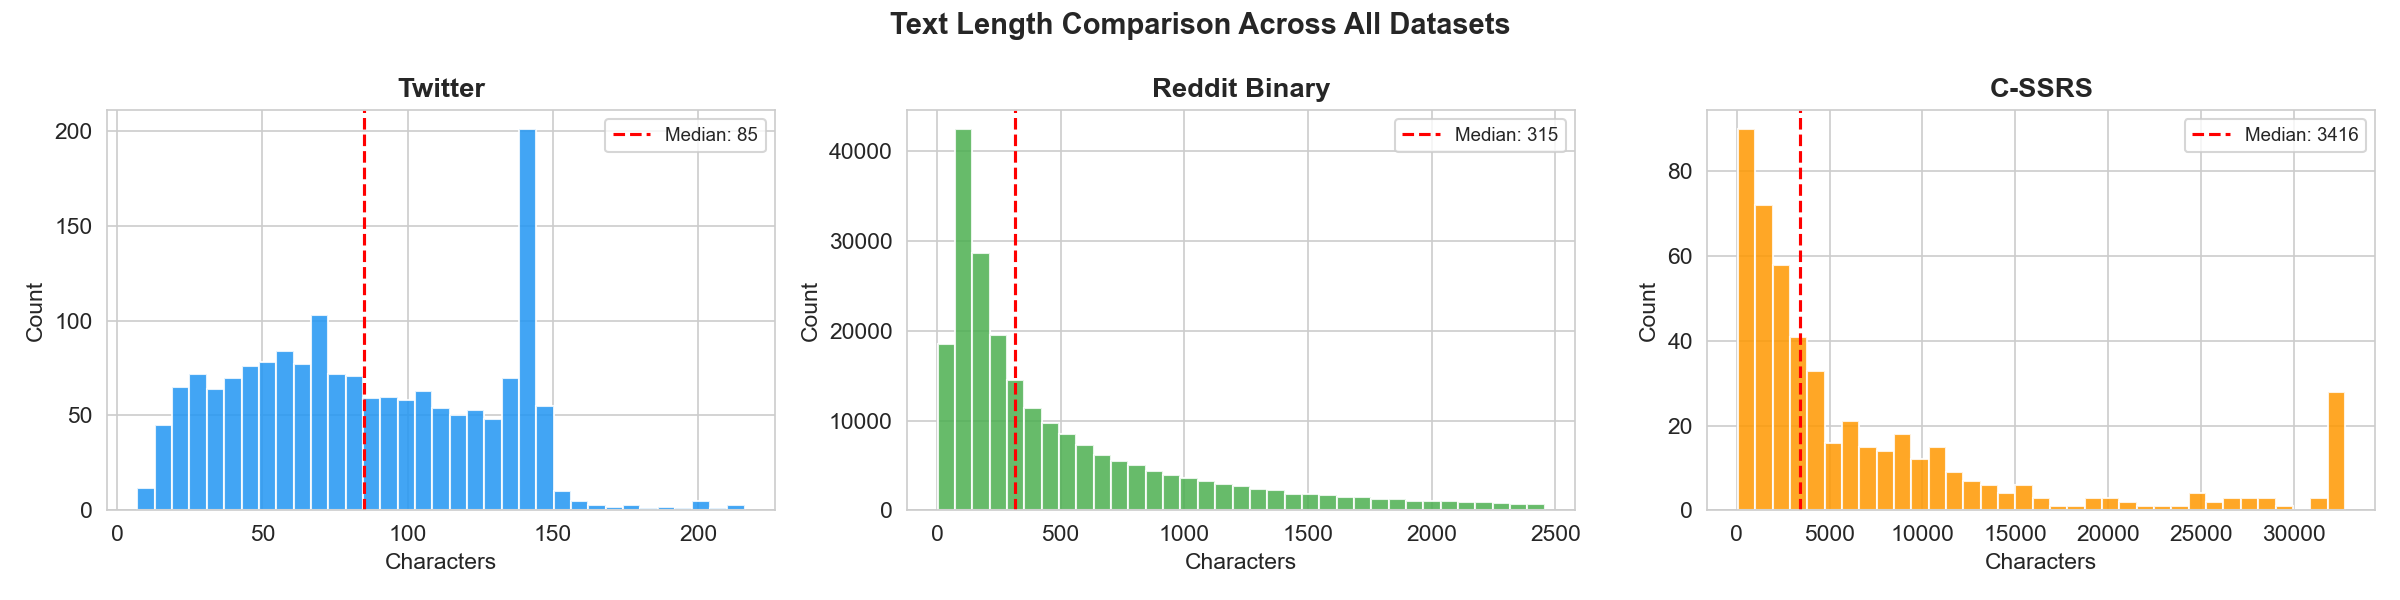
\includegraphics[width=0.95\textwidth]{04_text_length_comparison}
\caption{Text length distribution (character count) across all four datasets. Twitter and Russian VK have short median lengths ($\sim$85 and $\sim$250 characters respectively); C-SSRS posts are substantially longer ($\sim$3,400 characters median). This 40$\times$ range directly affects model selection.}
\label{fig:text_length}
\end{figure}

The text length variation across datasets turned out to be one of the most important factors in the whole project. Twitter posts are very short (often under 140 characters), which means models have very little context to work with. C-SSRS is at the other extreme — posts are essentially full paragraphs, with detailed descriptions of the poster's mental state. Russian VK sits in the middle. This range directly affects how well different models perform: TF-IDF handles short texts reasonably well, but transformers with their contextual representations become much more valuable as text gets longer and more complex.

\subsection{Per-Dataset EDA}

\begin{figure}[H]
\centering
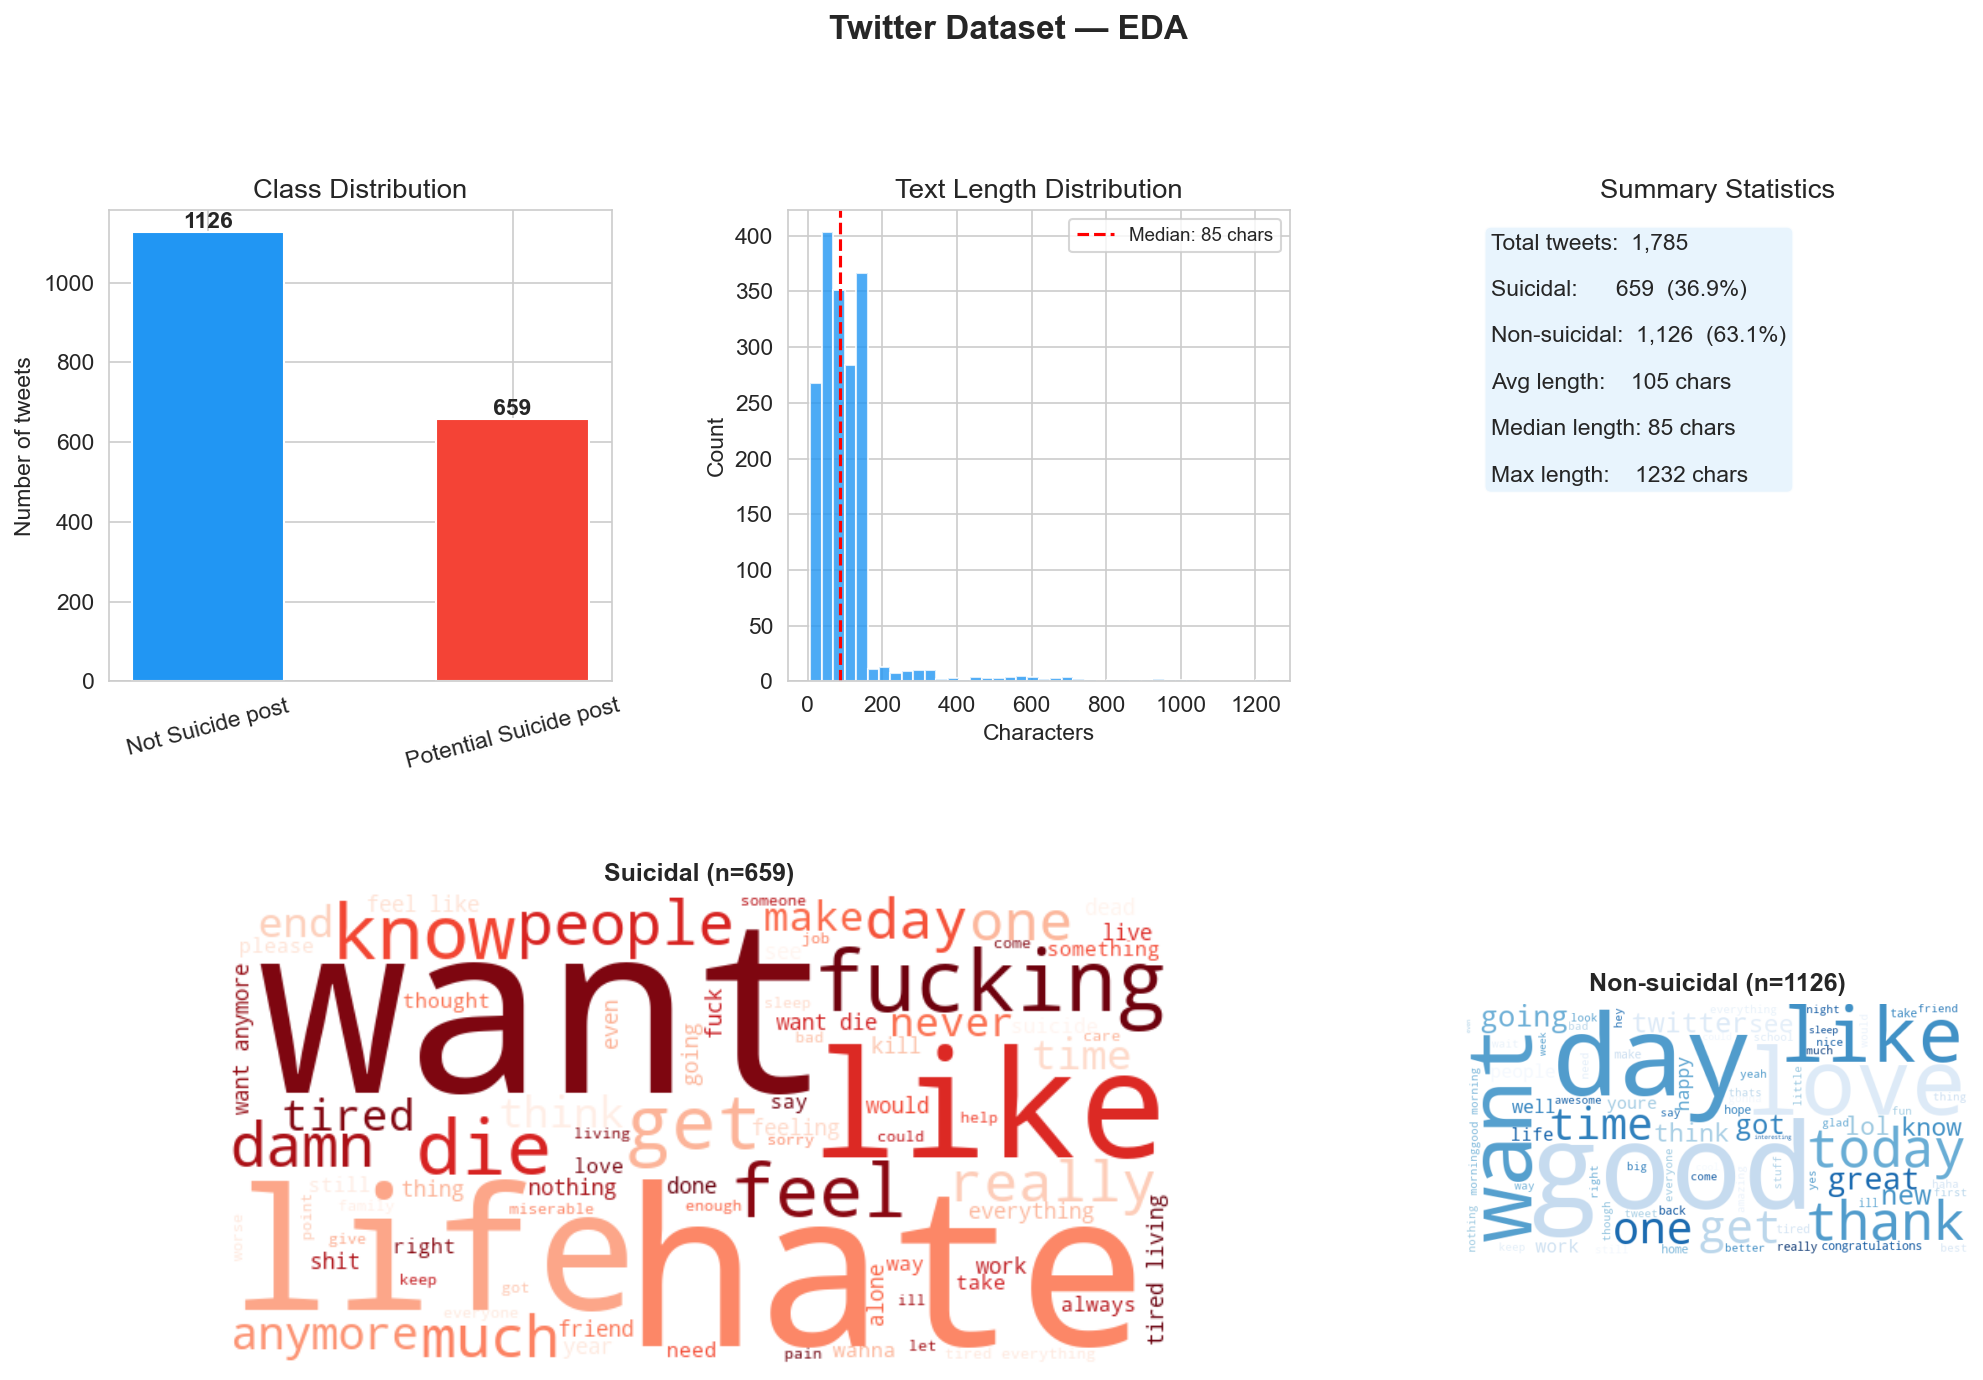
\includegraphics[width=\textwidth]{01_twitter_eda}
\caption{Twitter dataset: class distribution, text length by class, and word clouds for suicidal (top) and non-suicidal (bottom) posts. Explicit self-harm vocabulary is clearly visible in the suicidal word cloud.}
\label{fig:twitter_eda}
\end{figure}

What immediately stands out from the Twitter word cloud is how direct the suicidal class vocabulary is — words like \textit{kill}, \textit{life}, \textit{want} appear together in ways that are quite unambiguous. This is a bit different from what I expected; I thought social media users would express distress more indirectly. The class imbalance (37\% suicidal) is relatively mild but still enough to matter for models without class balancing.

\begin{figure}[H]
\centering
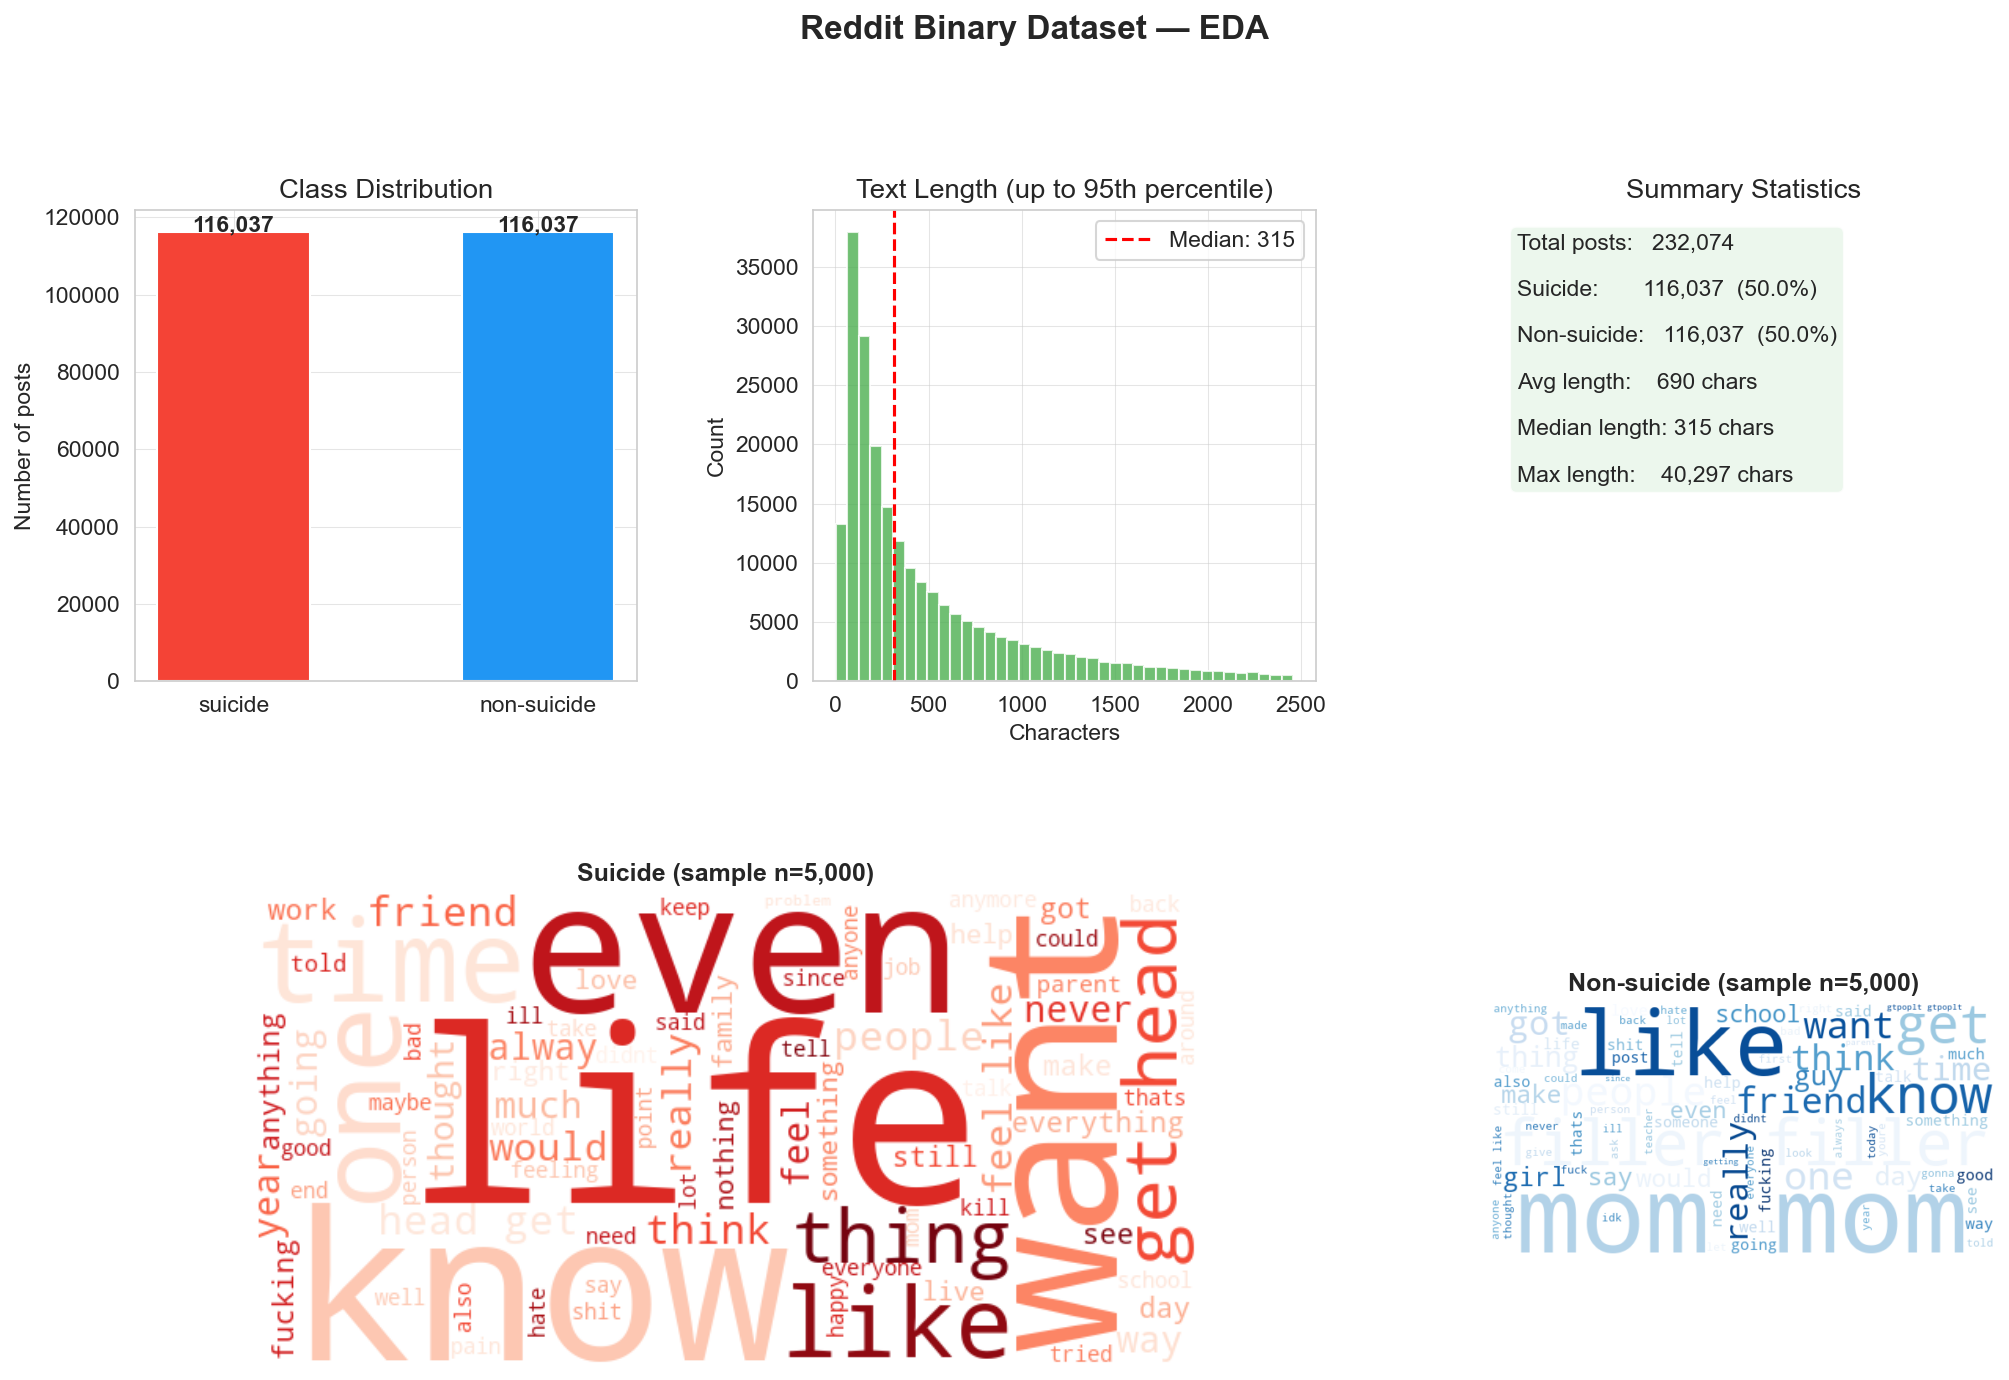
\includegraphics[width=\textwidth]{02_reddit_binary_eda}
\caption{Reddit Binary dataset: perfectly balanced classes, medium text lengths, and overlapping but distinguishable vocabulary between classes.}
\label{fig:reddit_eda}
\end{figure}

Reddit is the ideal benchmark dataset in many ways — 232,000 posts, perfect 50/50 balance, and enough text length per post that models have something to work with. The vocabulary overlap between classes is larger than Twitter though, which makes the task harder despite the clean class distribution. This is probably why classical ML still does well here: the lexical signal is strong enough for TF-IDF to capture.

\begin{figure}[H]
\centering
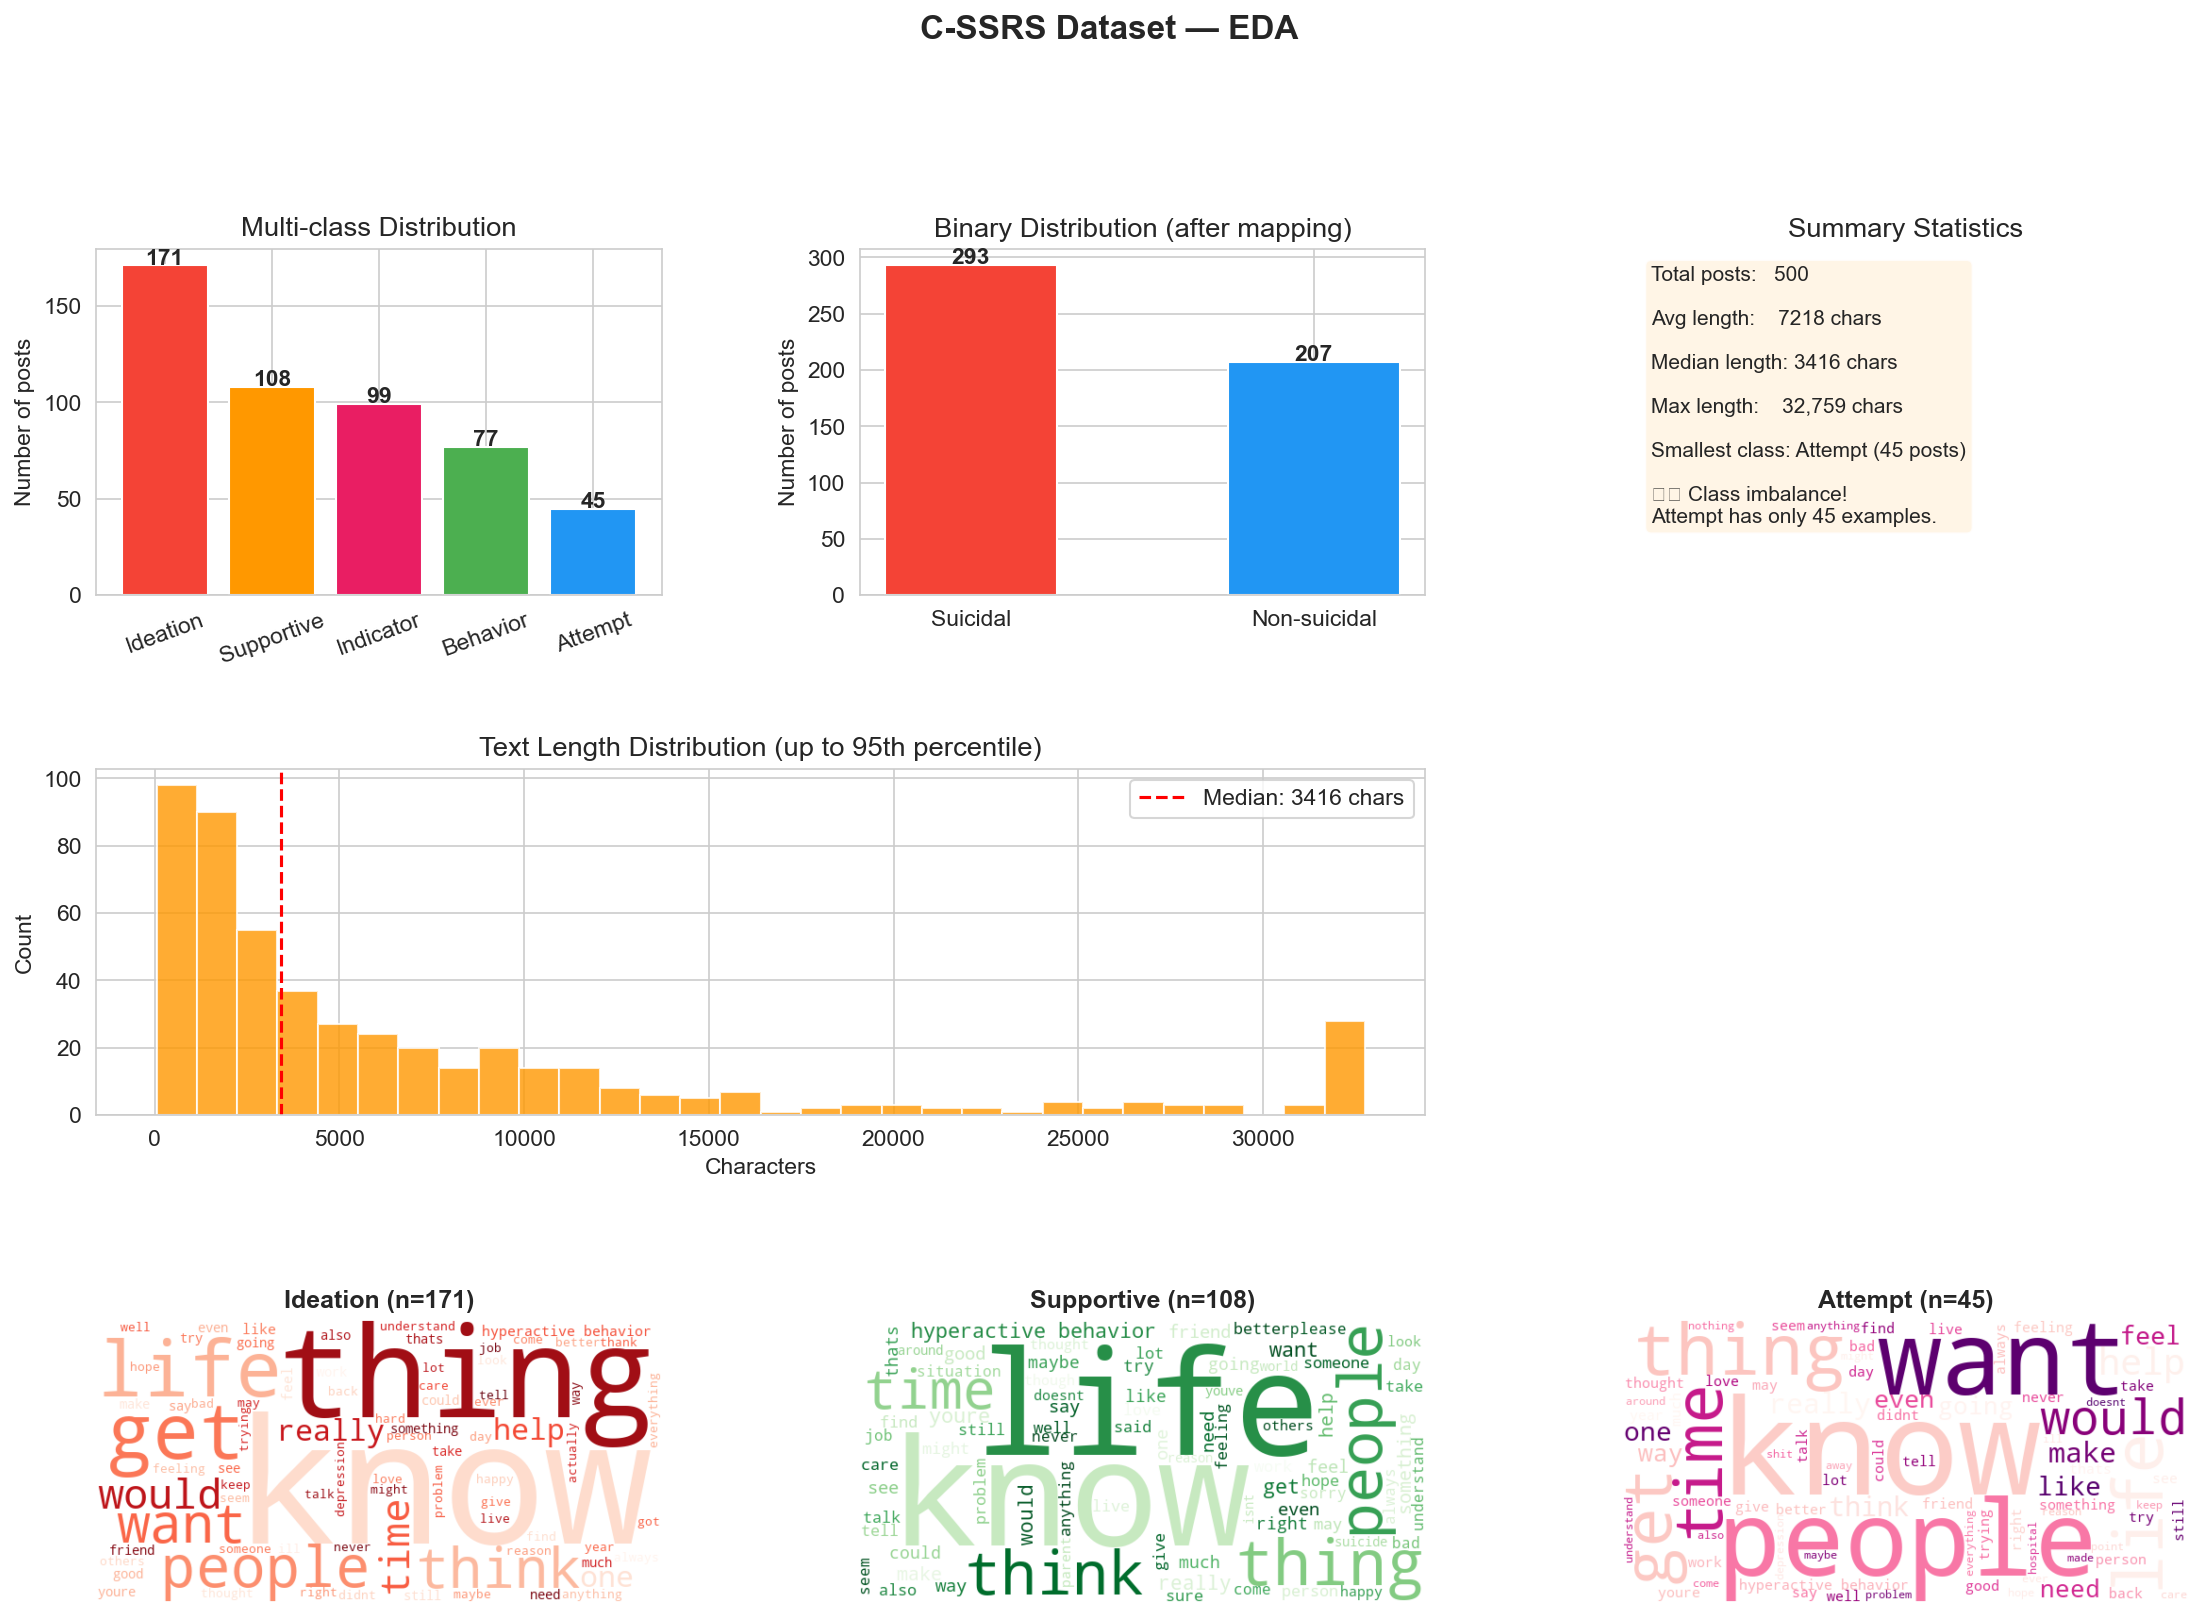
\includegraphics[width=\textwidth]{03_cssrs_eda}
\caption{C-SSRS dataset: severe class imbalance ($\sim$9\% minority), very long texts, and complex clinical language requiring contextual understanding.}
\label{fig:cssrs_eda}
\end{figure}

C-SSRS is by far the hardest dataset in this benchmark — 500 samples total, with only around 9\% belonging to the positive class. The long texts actually contain rich clinical language, but the data scarcity means most models struggle to generalise. It is worth noting that the original C-SSRS annotation scheme used five classes \citep{gaur2019knowledge}; I collapsed them into binary for comparability with the other datasets. This means the minority class here captures a range of severity levels (ideation, behaviour, attempt) and is not necessarily coherent as a single category.

\begin{figure}[H]
\centering
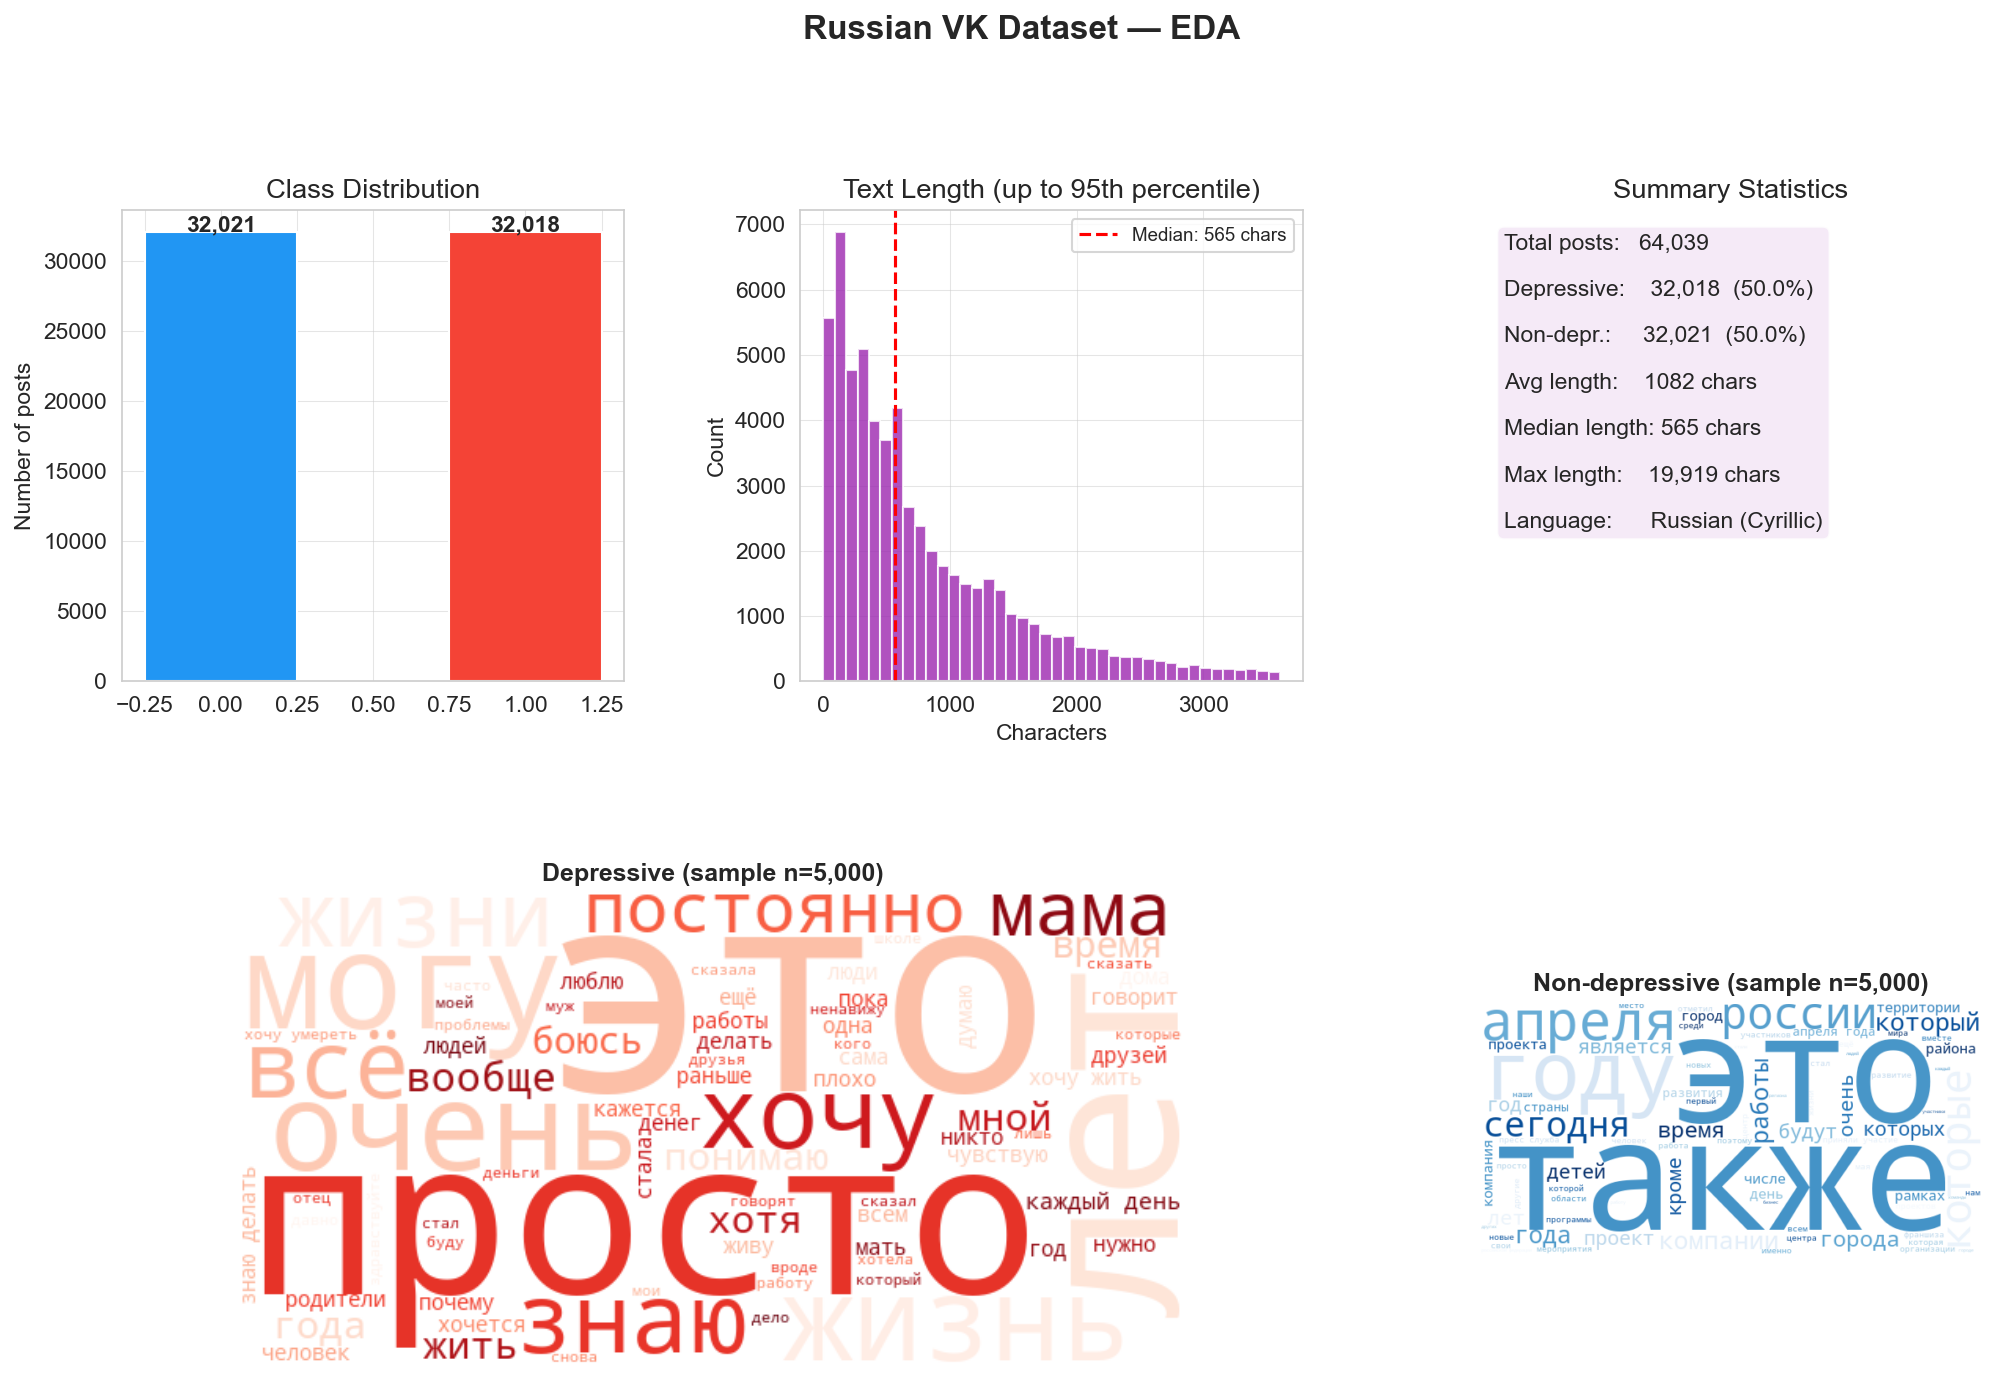
\includegraphics[width=\textwidth]{05_russian_vk_eda}
\caption{Russian VK dataset: balanced classes, short-to-medium texts, and Russian-language vocabulary characteristic of emotional and depressive expression on social media.}
\label{fig:vk_eda}
\end{figure}

The Russian VK dataset has the best properties from a machine learning perspective: 64,039 posts, perfect class balance, and distinctive enough vocabulary between classes that even TF-IDF achieves near-perfect F1. The downside — which SHAP analysis later revealed — is that the data has temporal and geographic artifacts from the scraping process. Models trained on this data are learning something real about depressive language, but also partially learning when and where the data was collected.

%=============================================================
\chapter{Methodology}
\label{ch:method}
%=============================================================

\section{Preprocessing}

\subsection{Classical ML Preprocessing}

For TF-IDF-based models, text is processed through the following pipeline:
\begin{enumerate}
    \item Lowercasing (English only)
    \item URL and mention removal
    \item Special character removal
    \item Stopword removal (NLTK English stopwords; Snowball Russian stopwords)
    \item Lemmatisation (WordNetLemmatizer for English; no lemmatiser applied for Russian)
\end{enumerate}

\textbf{Critical Russian-specific step:} A Cyrillic-only filter \texttt{[\^{}\textbackslash u0400-\textbackslash u04FF\textbackslash s]} removes all non-Cyrillic characters from Russian text. This step was added after SHAP analysis revealed that English words (e.g., \textit{depression}, \textit{twitter}) were leaking into Russian TF-IDF features and acting as spurious predictors (see Section~\ref{sec:shap_artifacts}).

\subsection{Transformer Preprocessing}

For BERT-family models, raw text is passed directly to the HuggingFace tokenizer with:
\begin{itemize}
    \item \texttt{max\_length=128} tokens with truncation and padding
    \item Model-specific tokenizer (\texttt{bert-base-uncased}, \texttt{bert-base-multilingual-cased}, \texttt{xlm-roberta-base})
\end{itemize}

\section{Model Architectures}

\subsection{Classical ML}

Three TF-IDF-based pipelines are used:
\begin{itemize}
    \item \textbf{Logistic Regression (LR):} \texttt{max\_iter=1000}, \texttt{class\_weight='balanced'}
    \item \textbf{Linear SVM:} LinearSVC with \texttt{class\_weight='balanced'}, \texttt{max\_iter=2000}
    \item \textbf{Random Forest (RF):} 200 estimators, \texttt{class\_weight='balanced'}
\end{itemize}
TF-IDF uses \texttt{max\_features=10000}, \texttt{ngram\_range=(1,2)}.

\subsection{Deep Learning}

Three recurrent architectures are implemented in PyTorch:
\begin{itemize}
    \item \textbf{LSTM:} single-layer, hidden size 128, pre-trained GloVe embeddings (100d), dropout 0.3
    \item \textbf{BiLSTM:} bidirectional LSTM, hidden size 128 per direction, same embeddings
    \item \textbf{GRU:} single-layer GRU, hidden size 128
\end{itemize}
All models use Adam optimiser (\texttt{lr=1e-3}), batch size 64, early stopping with patience 3.

\subsection{Transformer Models}

Three HuggingFace models are fine-tuned:
\begin{itemize}
    \item \textbf{BERT:} \texttt{bert-base-uncased} — English datasets only
    \item \textbf{mBERT:} \texttt{bert-base-multilingual-cased} — Russian VK
    \item \textbf{XLM-RoBERTa:} \texttt{xlm-roberta-base} — Russian VK and zero-shot transfer
\end{itemize}
Training: AdamW optimiser, \texttt{lr=2e-5}, warmup over 10\% of steps, 3 epochs, batch size 16. Best checkpoint selected by validation F1.

\section{Zero-Shot Cross-Lingual Transfer}

For the zero-shot experiment, XLM-RoBERTa is trained entirely on English Reddit data (20,000 posts) and evaluated directly on Russian VK test data (12,808 posts) without any Russian-language fine-tuning. This setup tests whether multilingual pre-training alone is sufficient for cross-lingual generalisation.

\section{Evaluation Protocol}

\begin{itemize}
    \item \textbf{Split:} Stratified 80/20 train/test, \texttt{random\_state=42} throughout
    \item \textbf{Primary metric:} Weighted F1-score (handles class imbalance correctly)
    \item \textbf{Additional metrics:} Accuracy, precision, recall, ROC-AUC (where applicable)
    \item All results saved as JSON files to \texttt{results/metrics/}
\end{itemize}

%=============================================================
\chapter{Classical ML Results}
\label{ch:ml}
%=============================================================

\section{Results}

Table~\ref{tab:ml_results} presents the weighted F1-scores for all three classical ML models across all four datasets.

\begin{table}[H]
\centering
\caption{Classical ML weighted F1-scores. Best per dataset in \textbf{bold}.}
\label{tab:ml_results}
\begin{tabular}{lcccc}
\toprule
\textbf{Model} & \textbf{Twitter (EN)} & \textbf{Reddit (EN)} & \textbf{C-SSRS (EN)} & \textbf{Russian VK (RU)} \\
\midrule
Logistic Regression & 0.8839 & 0.9411 & 0.7060 & 0.9899 \\
Linear SVM          & 0.9194 & 0.9396 & \textbf{0.7270} & \textbf{0.9948} \\
Random Forest       & \textbf{0.9349} & 0.9083 & 0.6476 & 0.9804 \\
\bottomrule
\end{tabular}
\end{table}

\begin{figure}[H]
\centering
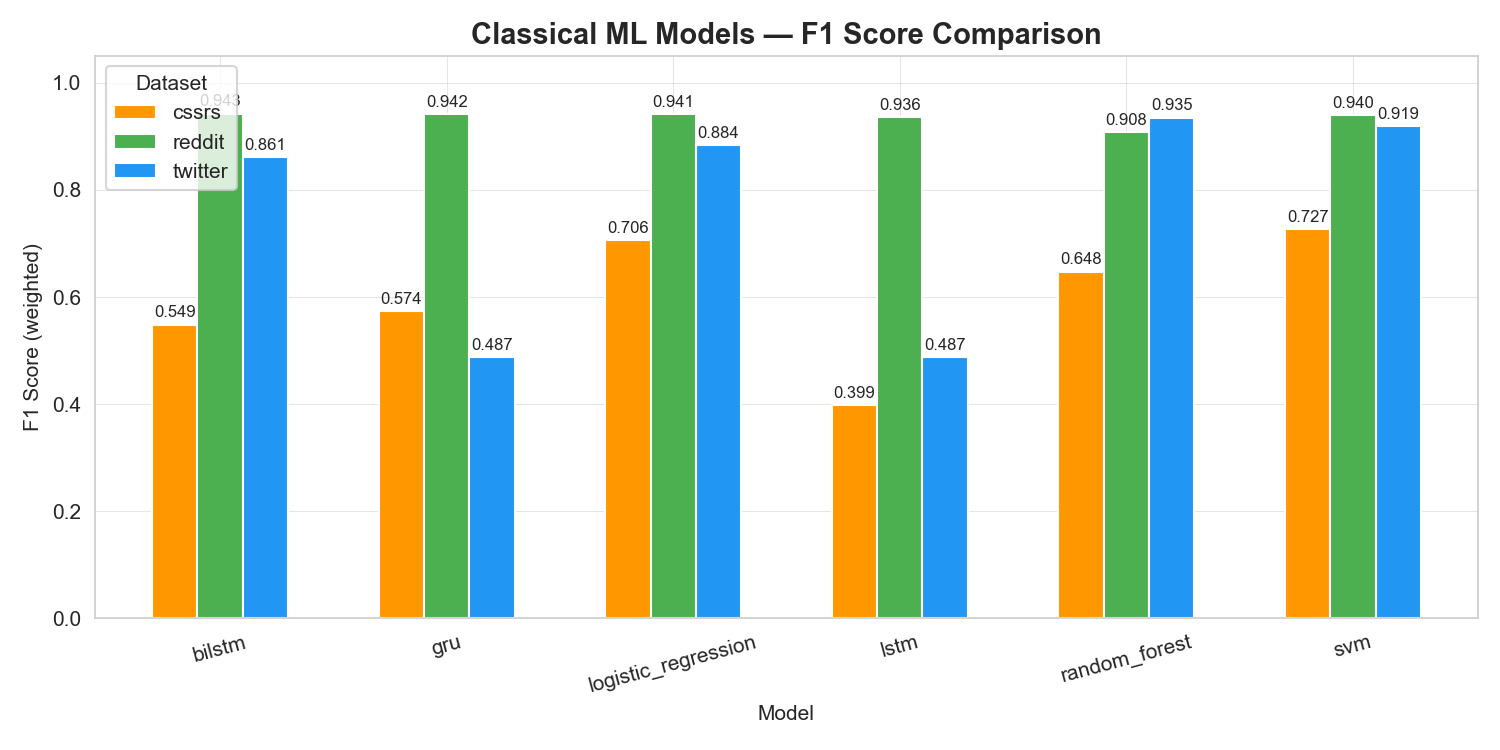
\includegraphics[width=0.9\textwidth]{ml_f1_comparison}
\caption{Weighted F1-score comparison across all classical ML models and datasets.}
\label{fig:ml_f1}
\end{figure}

The most striking thing in this chart is not which model wins — it is how much the dataset matters. Reddit and Russian VK both achieve F1 above 0.90 across all three models, while C-SSRS struggles to get above 0.73 even with the best model. The gap between datasets is around five times larger than the gap between models within any one dataset. This suggests that for this type of problem, collecting more or better-labelled data matters more than picking the right algorithm.

\begin{figure}[H]
\centering
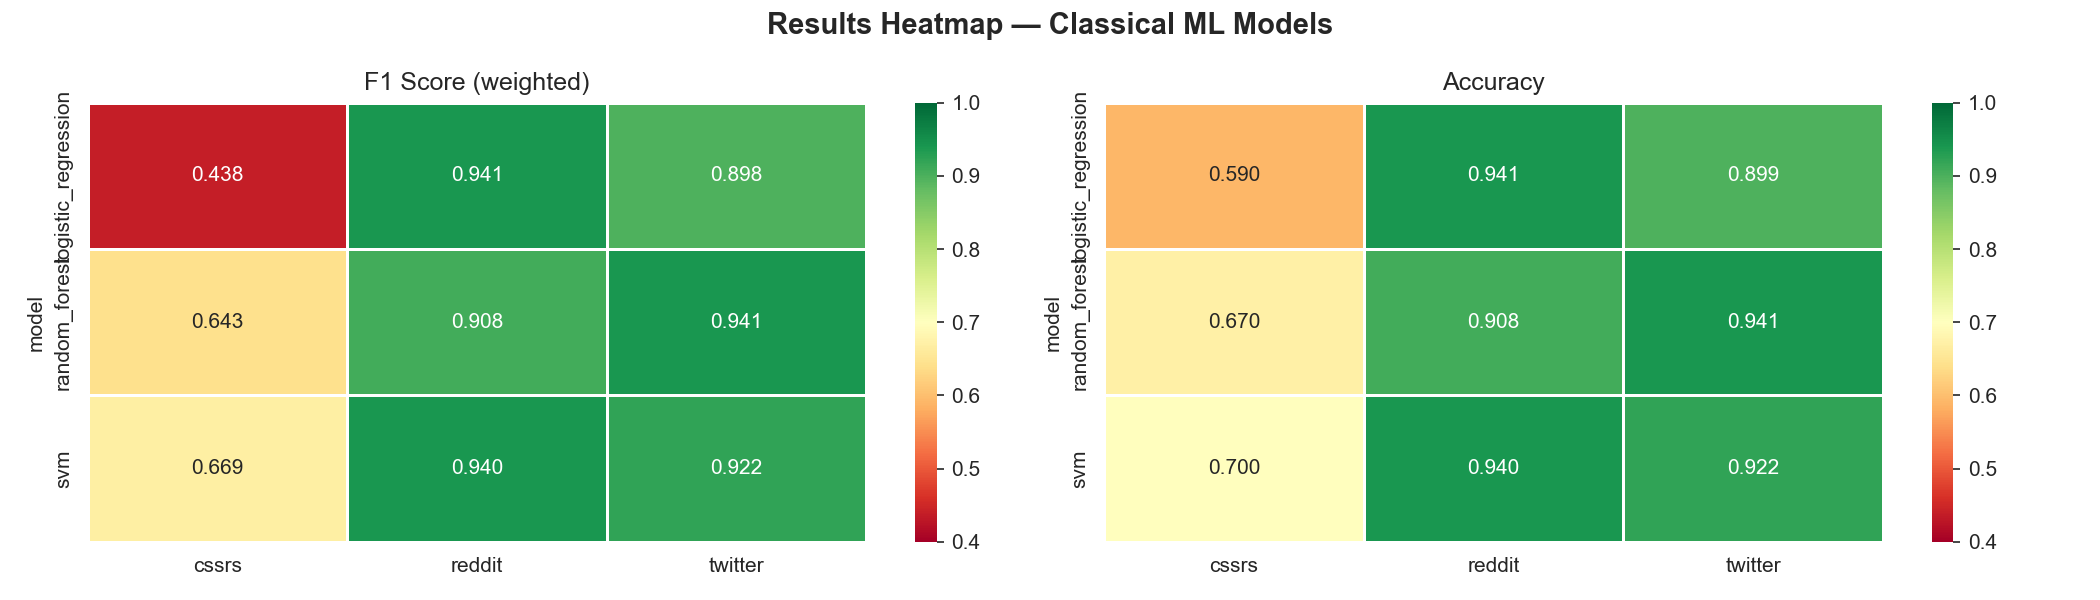
\includegraphics[width=0.75\textwidth]{ml_heatmap}
\caption{Results heatmap for classical ML models. Dataset difficulty dominates model differences.}
\label{fig:ml_heatmap}
\end{figure}

The heatmap makes the dataset-driven pattern even clearer — the columns (datasets) are much more different from each other than the rows (models). The dark column for C-SSRS stands out immediately. Interestingly, Random Forest is the best on Twitter but the worst on Reddit and C-SSRS. This is probably because RF is good at capturing non-linear combinations of features, which matters more with limited data, but it loses its advantage when the text is longer and LR's regularisation helps more.

\section{Confusion Matrices}

\begin{figure}[H]
\centering
\begin{subfigure}[b]{0.48\textwidth}
    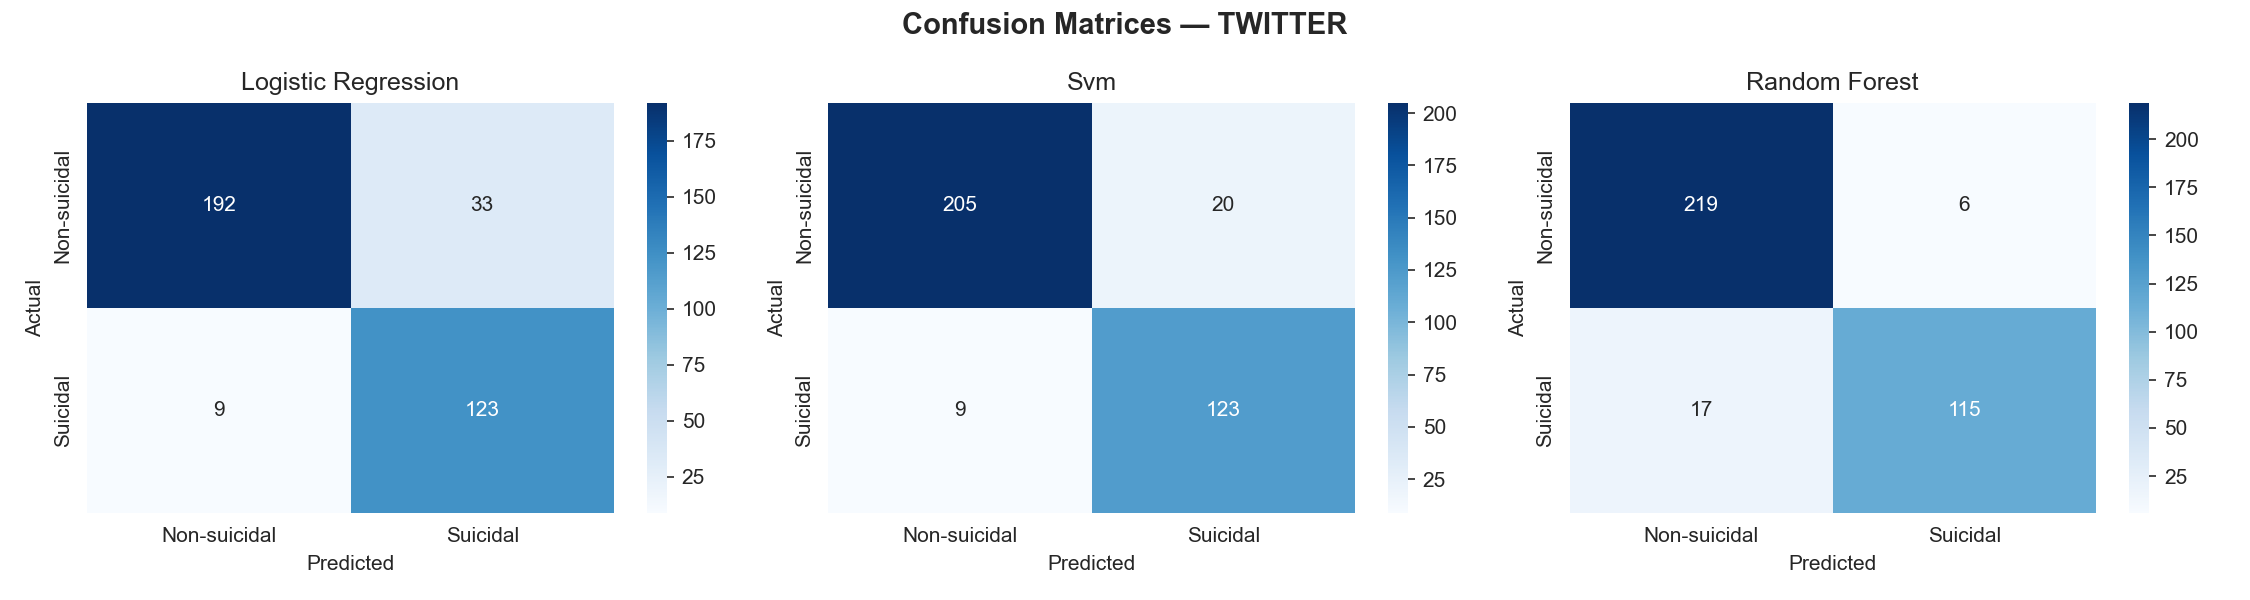
\includegraphics[width=\textwidth]{cm_twitter}
    \caption{Twitter — best model (Random Forest)}
\end{subfigure}
\hfill
\begin{subfigure}[b]{0.48\textwidth}
    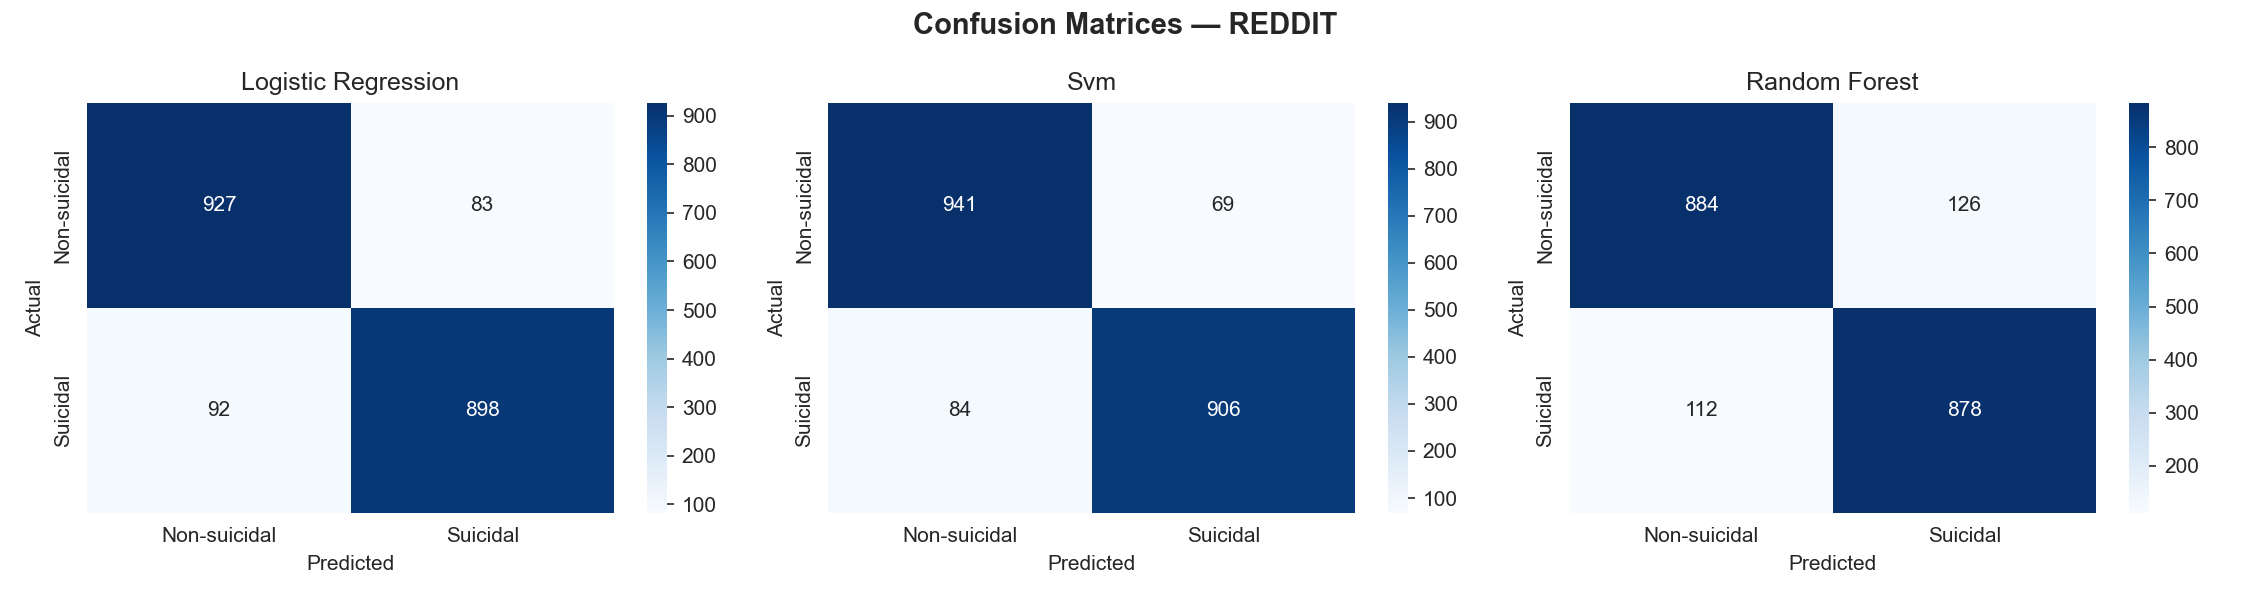
\includegraphics[width=\textwidth]{cm_reddit}
    \caption{Reddit — best model (Logistic Regression)}
\end{subfigure}
\caption{Confusion matrices for best classical ML models on Twitter and Reddit datasets.}
\label{fig:cm_ml}
\end{figure}

The Twitter matrix shows a fairly symmetric error pattern — roughly equal false positives and false negatives — which makes sense given the moderate class imbalance. Reddit's matrix looks almost clean: 232k posts with strong lexical separation means the model rarely confuses the two classes. The false negatives are slightly higher than false positives in both cases, which is the safer error direction for a screening tool (not ideal, but better than missing half the positives).

\begin{figure}[H]
\centering
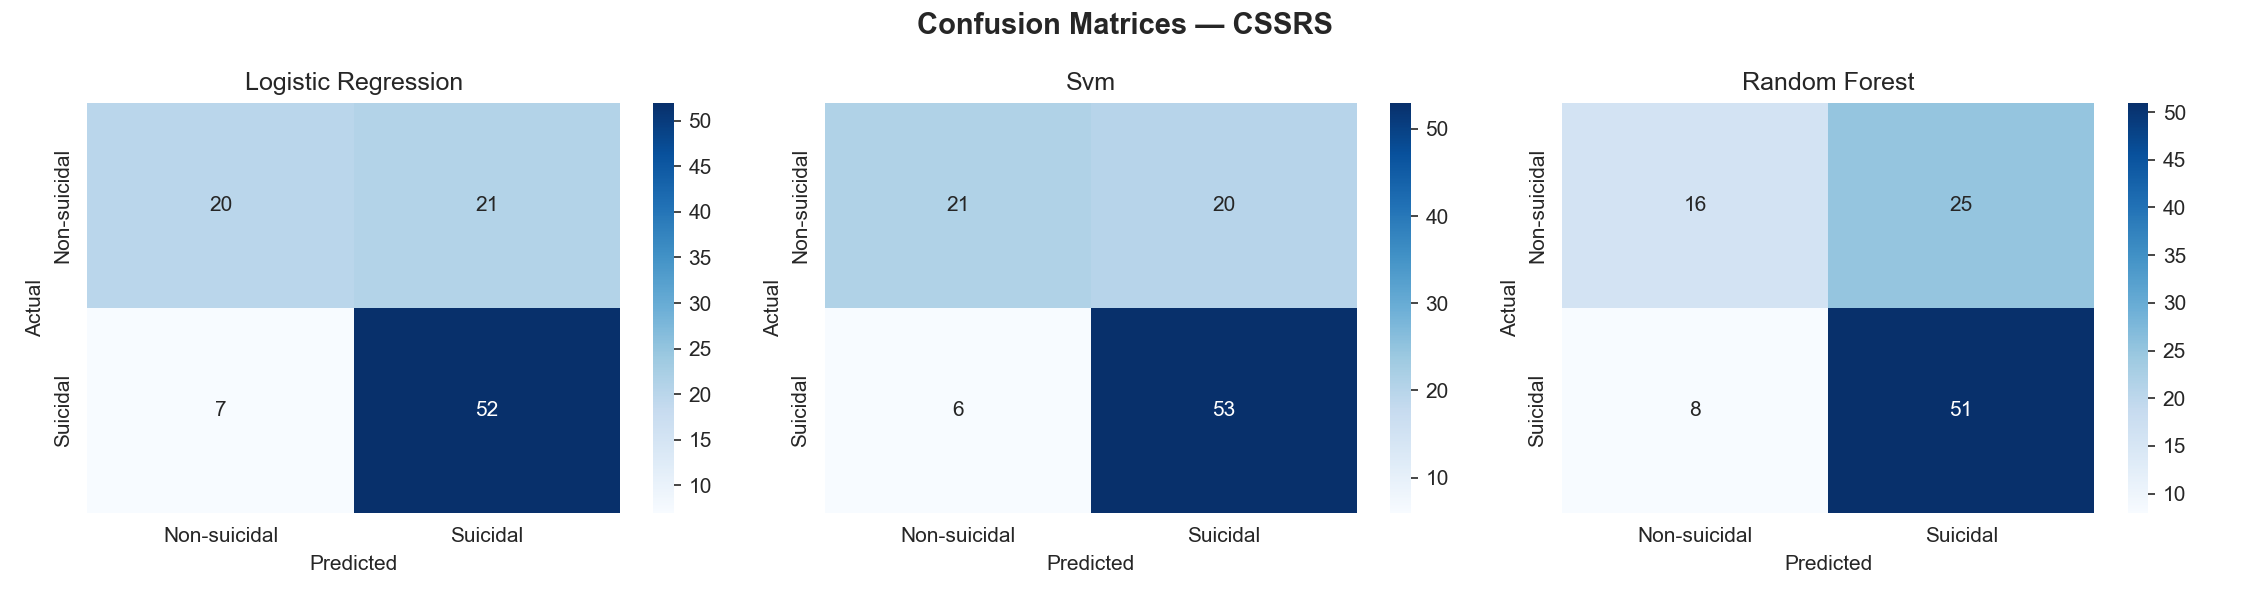
\includegraphics[width=0.52\textwidth]{cm_cssrs}
\caption{C-SSRS confusion matrix. Class imbalance is visible even after balanced class weighting.}
\label{fig:cm_cssrs}
\end{figure}

C-SSRS is the most revealing confusion matrix. Even with \texttt{class\_weight='balanced'}, the minority class (suicidal, $\sim$9\%) is still misclassified quite often. The model is clearly struggling with the limited data rather than any particular language pattern — with only 40 minority-class training examples, it can't generalise reliably. This is a case where more data would help far more than a better algorithm.

\section{Key Findings}

\begin{findingbox}[title={Finding 1 — No single model wins across all datasets}]
Random Forest is best on Twitter (F1=0.935), Logistic Regression on Reddit (F1=0.941), and SVM on C-SSRS (F1=0.727). Model selection must be dataset-specific.
\end{findingbox}

\begin{findingbox}[title={Finding 2 — Dataset difficulty dominates model differences}]
The best F1 on Reddit (0.941) vs C-SSRS (0.727) represents a 0.21-point gap — 5$\times$ larger than the gap between the best and worst model on any single dataset.
\end{findingbox}

\begin{findingbox}[title={Finding 3 — Class weight correction is critical for C-SSRS}]
Without \texttt{class\_weight='balanced'}, Logistic Regression fails entirely on C-SSRS (F1=0.44). After correction: F1=0.706, a gain of 27 percentage points.
\end{findingbox}

\section{LIME Analysis}

\begin{figure}[H]
\centering
\begin{subfigure}[b]{0.48\textwidth}
    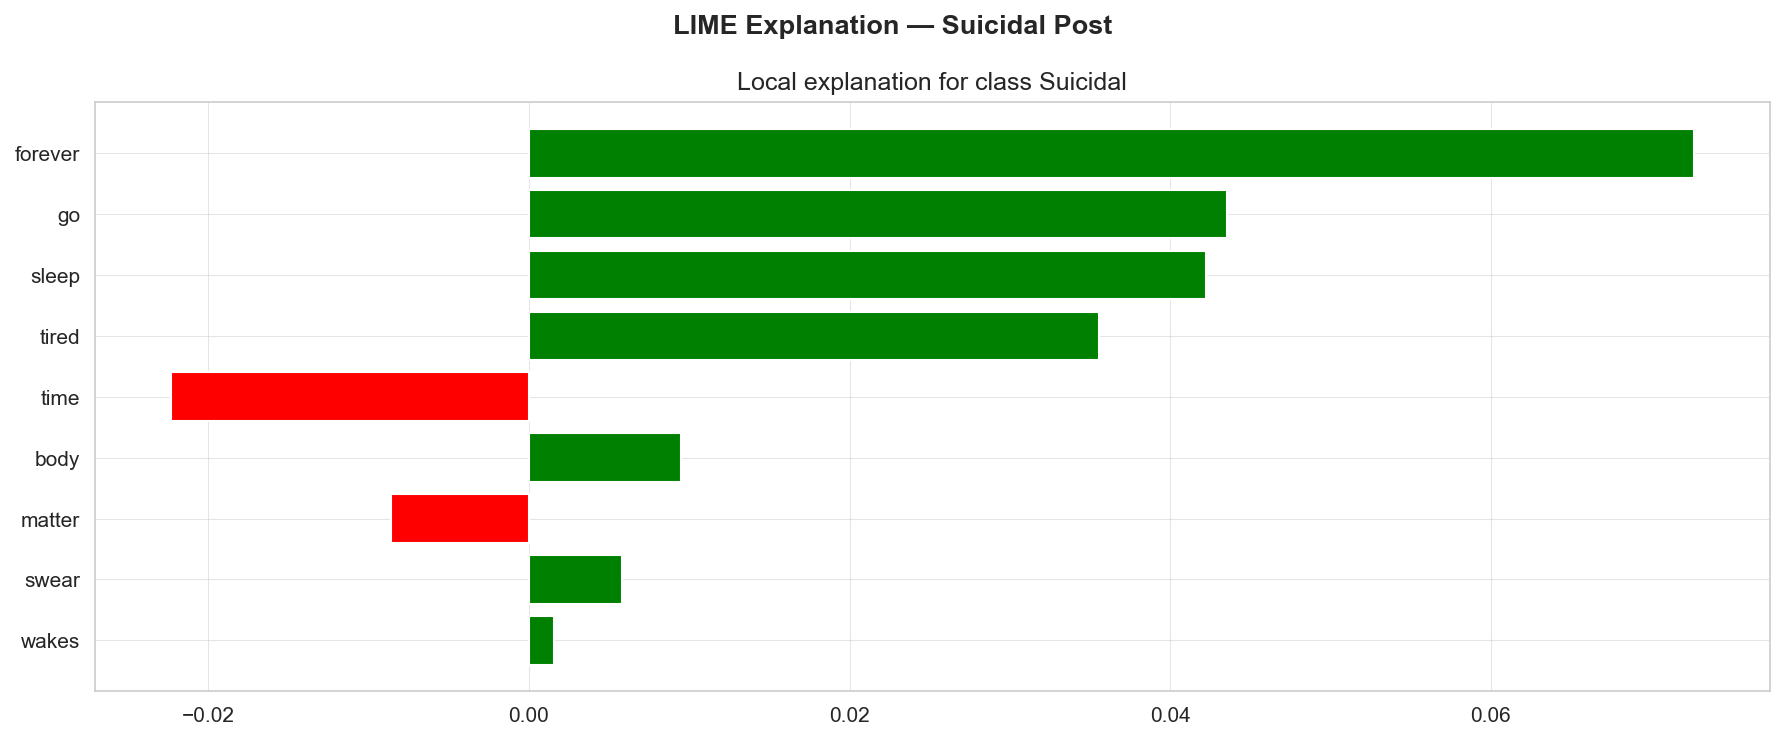
\includegraphics[width=\textwidth]{lime_suicidal_example}
    \caption{Suicidal post — top features include \textit{forever}, \textit{sleep}, \textit{tired}}
\end{subfigure}
\hfill
\begin{subfigure}[b]{0.48\textwidth}
    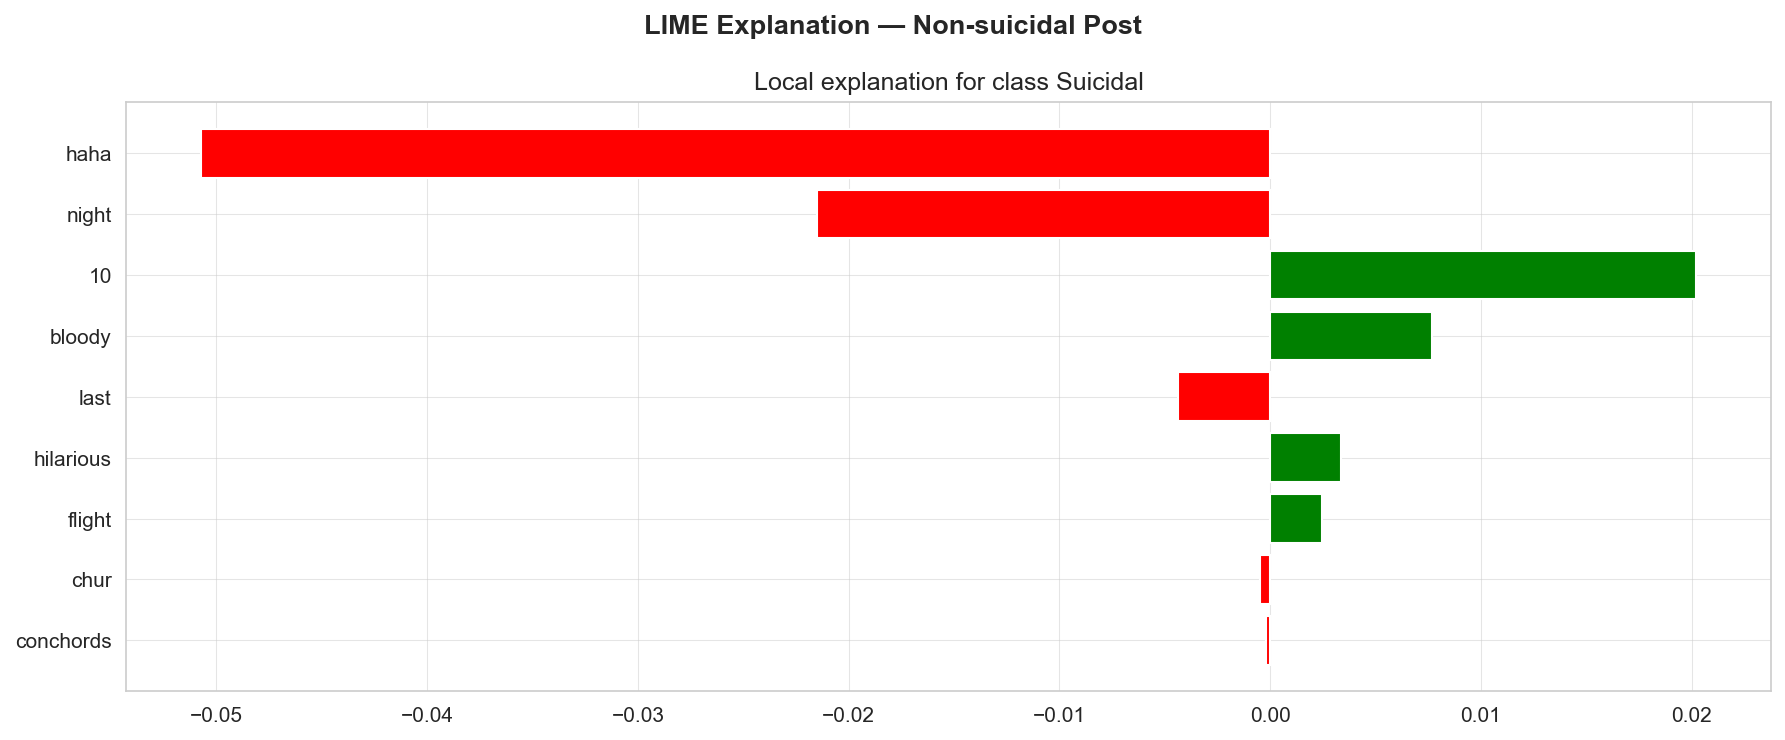
\includegraphics[width=\textwidth]{lime_non_suicidal_example}
    \caption{Non-suicidal post — features reflect everyday language}
\end{subfigure}
\caption{LIME explanations for Twitter SVM predictions. The model activates on clinically meaningful euphemistic vocabulary.}
\label{fig:lime_twitter}
\end{figure}

%=============================================================
\chapter{Deep Learning Results}
\label{ch:dl}
%=============================================================

\section{Results}

\begin{table}[H]
\centering
\caption{Deep learning weighted F1-scores. ❌ indicates model collapse (predicts majority class only).}
\label{tab:dl_results}
\begin{tabular}{lccc}
\toprule
\textbf{Model} & \textbf{Twitter (EN)} & \textbf{Reddit (EN)} & \textbf{C-SSRS (EN)} \\
\midrule
LSTM   & 0.49~❌ & 0.9364 & 0.3988 \\
BiLSTM & \textbf{0.8607} & \textbf{0.9425} & 0.5487 \\
GRU    & 0.49~❌ & 0.9415 & \textbf{0.5739} \\
\bottomrule
\end{tabular}
\end{table}

\begin{figure}[H]
\centering
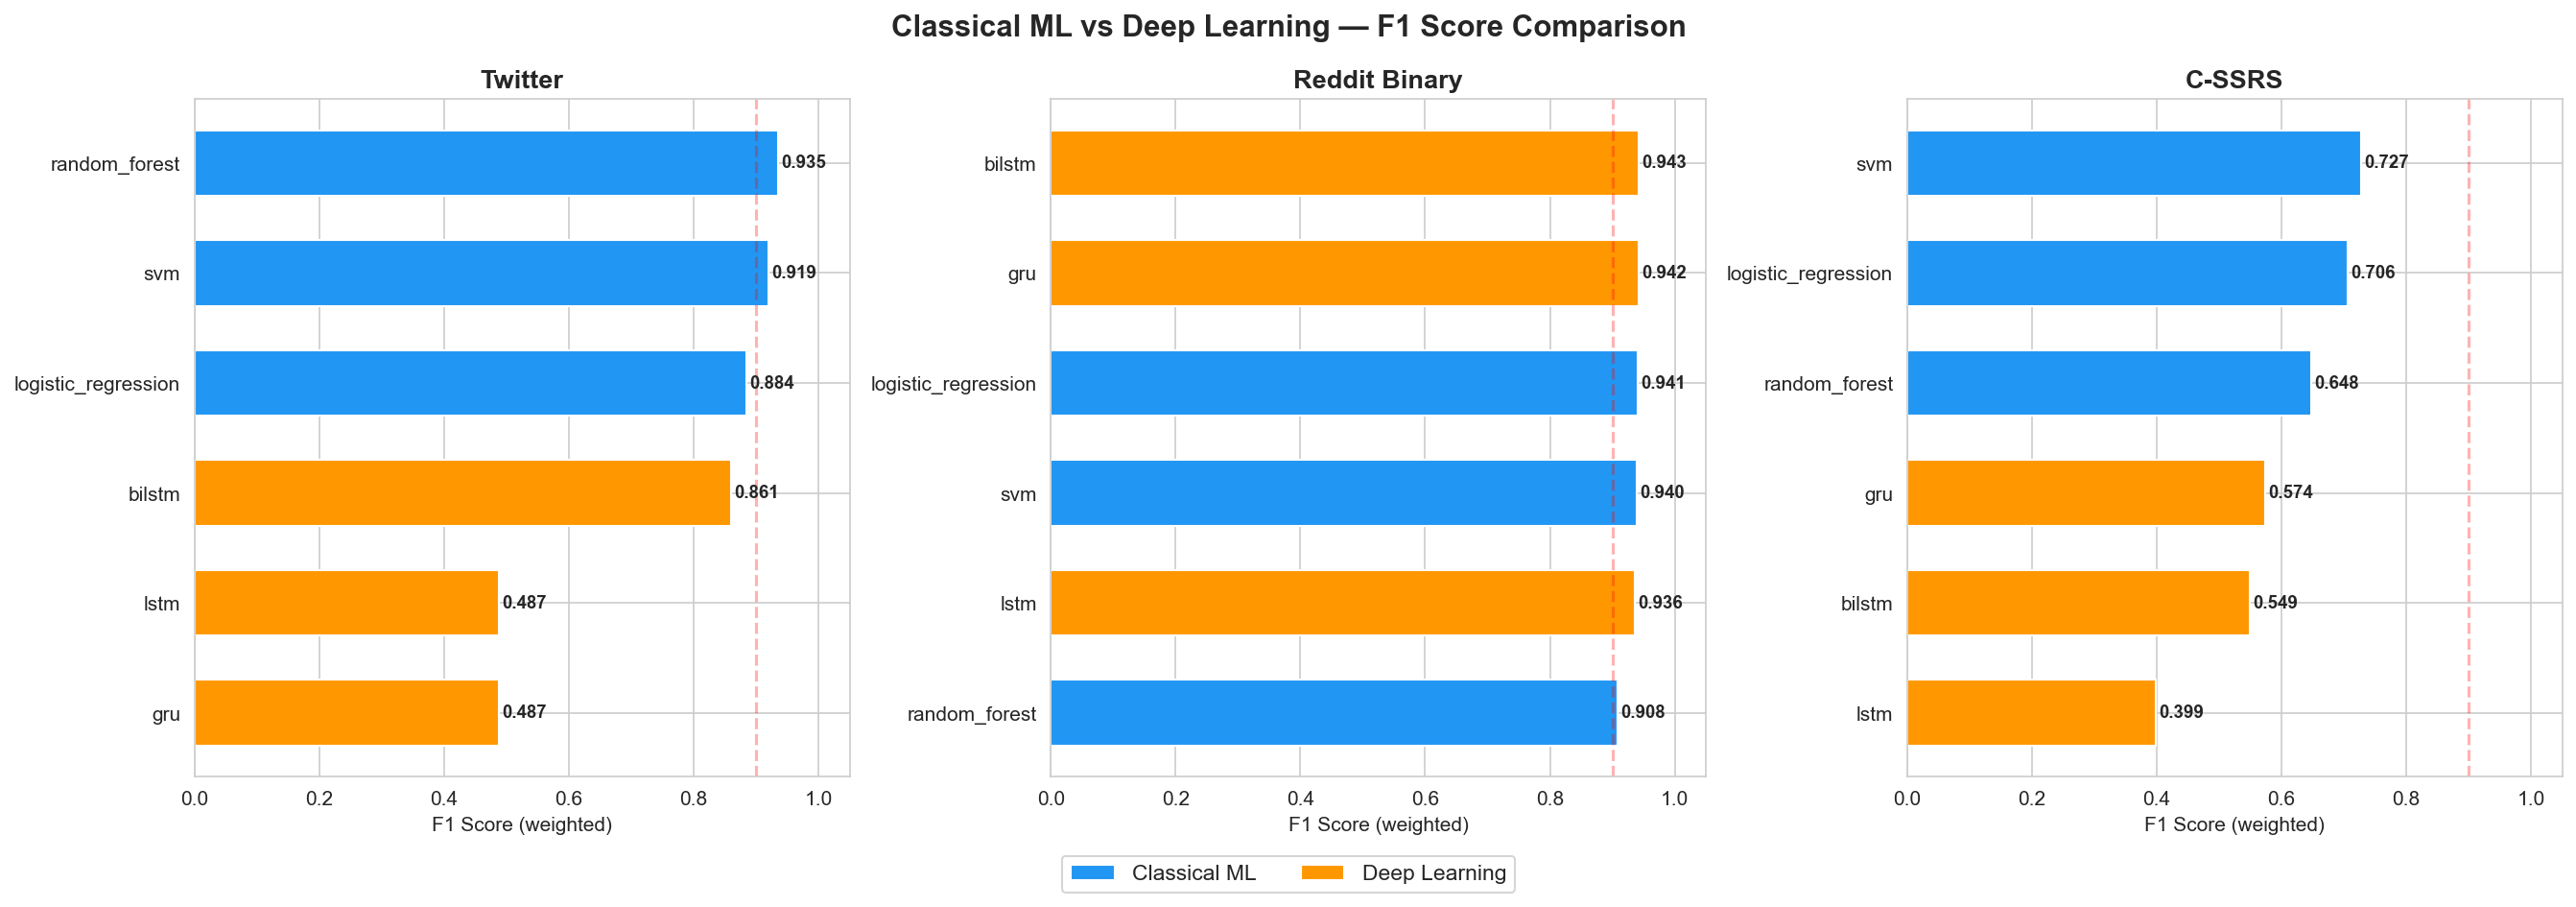
\includegraphics[width=0.9\textwidth]{ml_vs_dl_comparison}
\caption{Classical ML vs deep learning F1-scores per dataset. DL only wins on Reddit (232k posts).}
\label{fig:ml_vs_dl}
\end{figure}

This result surprised me more than almost anything in the thesis. I expected deep learning to be competitive across the board, but the comparison clearly shows it only wins on Reddit — the one dataset big enough to actually train a recurrent network properly. On Twitter, the DL models are dramatically worse (mainly due to LSTM/GRU collapse). On C-SSRS, they are also worse. The practical implication is that TF-IDF + classical ML should always be the baseline before investing in neural architectures.

\begin{figure}[H]
\centering
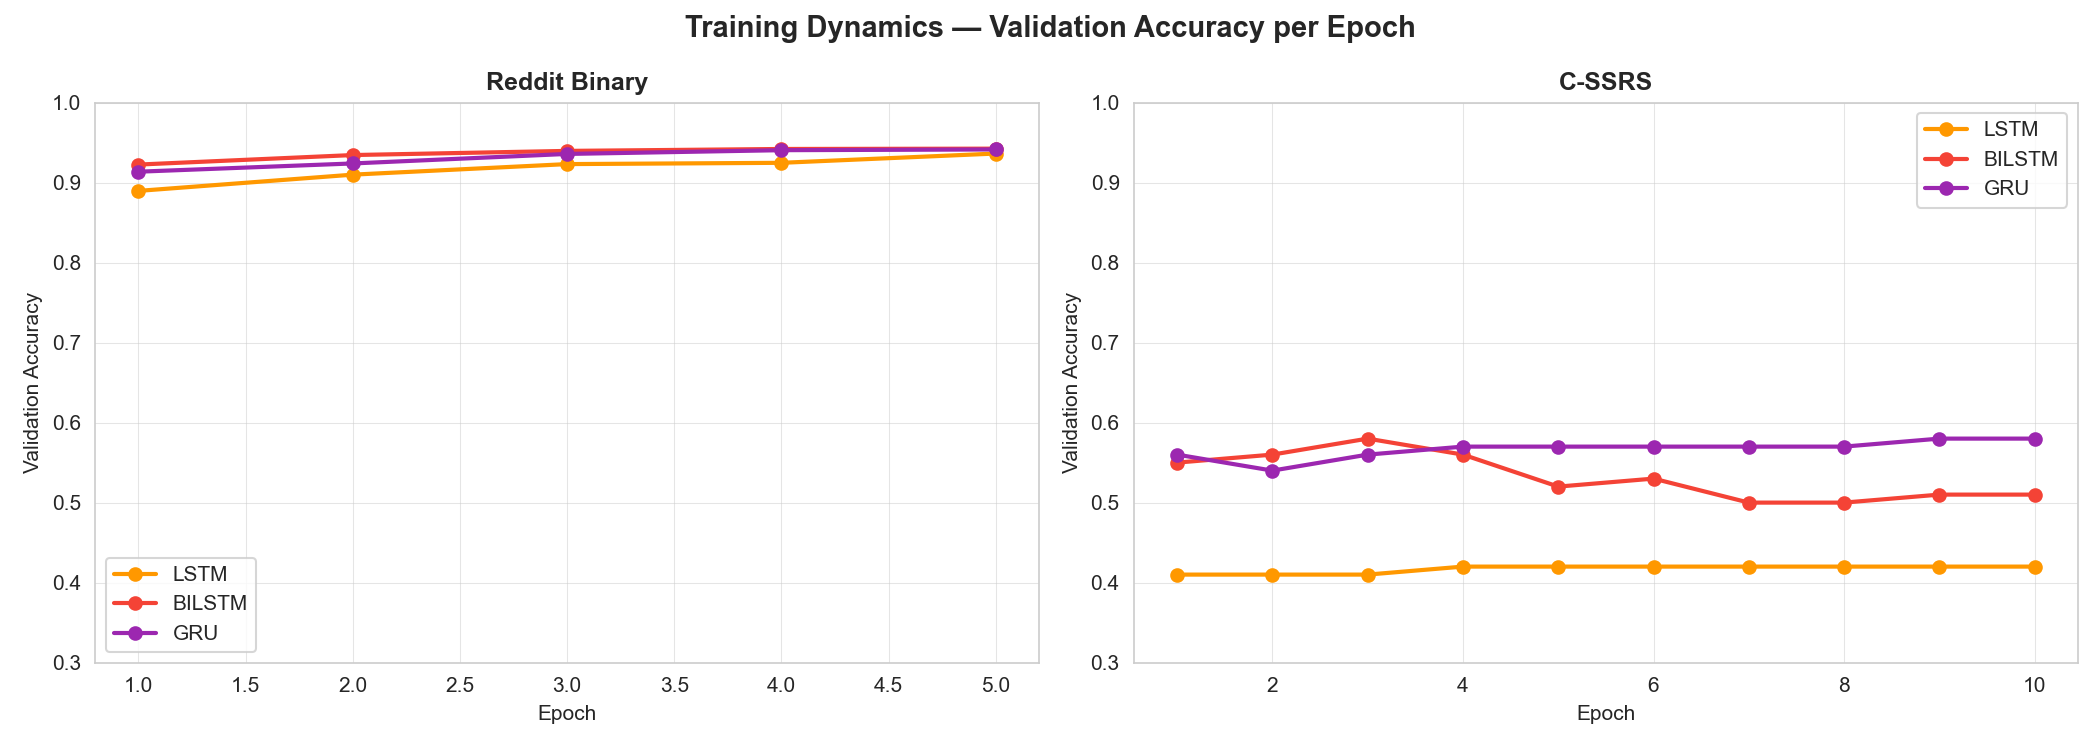
\includegraphics[width=0.9\textwidth]{dl_training_dynamics}
\caption{Training dynamics: validation accuracy per epoch for all three architectures. Reddit shows smooth convergence; C-SSRS shows high variance throughout training.}
\label{fig:dl_training}
\end{figure}

The training curves are quite telling. Reddit converges smoothly, which confirms the model is learning rather than memorising. C-SSRS, on the other hand, oscillates throughout — the validation accuracy jumps up and down between epochs, which is a classic sign of overfitting to a tiny training set. The model is essentially relearning the same few examples each epoch. This is why early stopping only helps marginally on C-SSRS.

\begin{figure}[H]
\centering
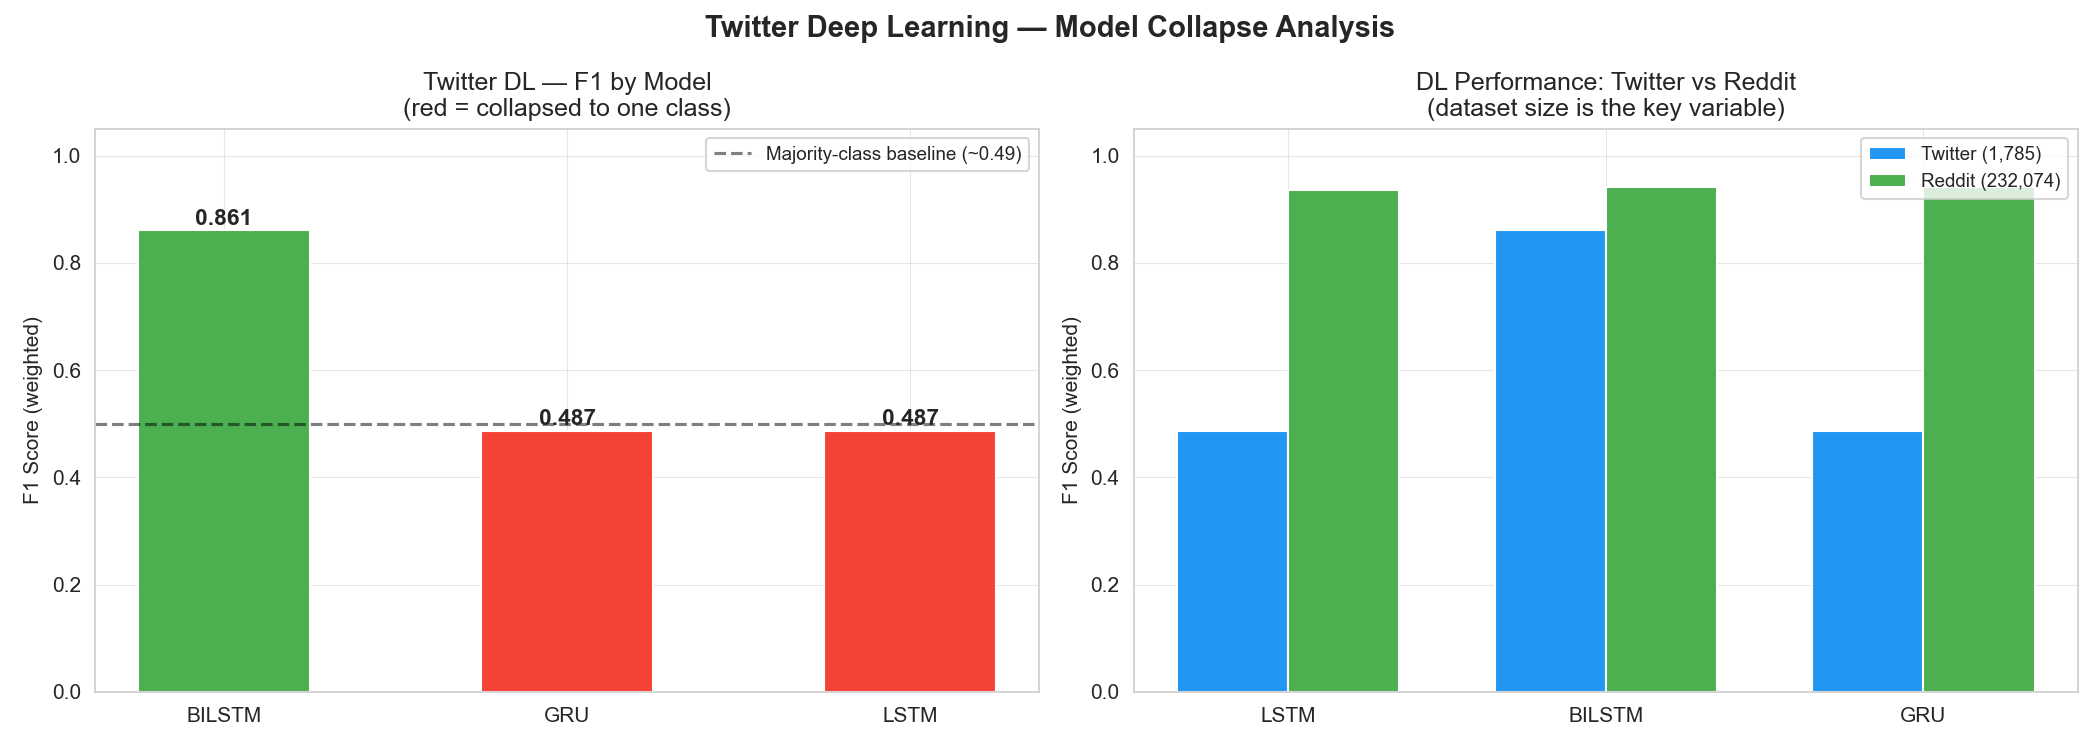
\includegraphics[width=0.75\textwidth]{twitter_dl_collapse}
\caption{LSTM and GRU collapse on Twitter: F1$\approx$0.49 (equivalent to predicting the majority class for all samples). BiLSTM avoids this failure mode.}
\label{fig:dl_collapse}
\end{figure}

The Twitter collapse is actually an interesting failure mode. LSTM and GRU both settle at F1$\approx$0.49 — which is exactly what you get if you predict the majority class (non-suicidal, 63\%) for every single example. The models never learn to identify the positive class. BiLSTM avoids this because bidirectional gradient flow doubles the effective training signal per token, which is apparently enough to overcome the 1,428-sample limitation. This threshold effect — where BiLSTM survives but LSTM fails — is a useful rule of thumb for very small datasets.

\section{Key Findings}

\begin{findingbox}[title={Finding 1 — LSTM and GRU collapse on Twitter}]
With only 1,428 training examples, LSTM and GRU never learn to predict the minority class (F1$\approx$0.49). BiLSTM achieves F1=0.861 on the same data because bidirectional gradient flow doubles the effective signal per token.
\end{findingbox}

\begin{findingbox}[title={Finding 2 — Classical ML outperforms DL on 2 of 3 datasets}]
ML average F1 on Twitter: 0.91 vs DL: 0.61. The minimum viable training size for randomly-initialised RNNs is approximately 5,000--10,000 samples; BiLSTM can function with $\sim$1,500.
\end{findingbox}

%=============================================================
\chapter{BERT Results}
\label{ch:bert}
%=============================================================

\section{Results}

\begin{table}[H]
\centering
\caption{Transformer weighted F1-scores. Best English results in \textbf{bold}.}
\label{tab:bert_results}
\begin{tabular}{lcccc}
\toprule
\textbf{Model} & \textbf{Twitter (EN)} & \textbf{Reddit (EN)} & \textbf{C-SSRS (EN)} & \textbf{Russian VK (RU)} \\
\midrule
BERT (\texttt{bert-base-uncased})             & \textbf{0.9468} & \textbf{0.9653} & 0.7100 & --- \\
mBERT (\texttt{bert-base-multilingual-cased}) & ---             & ---             & ---    & 0.9920 \\
XLM-R (\texttt{xlm-roberta-base})             & ---             & ---             & ---    & \textbf{0.9942} \\
\bottomrule
\end{tabular}
\end{table}

\begin{figure}[H]
\centering
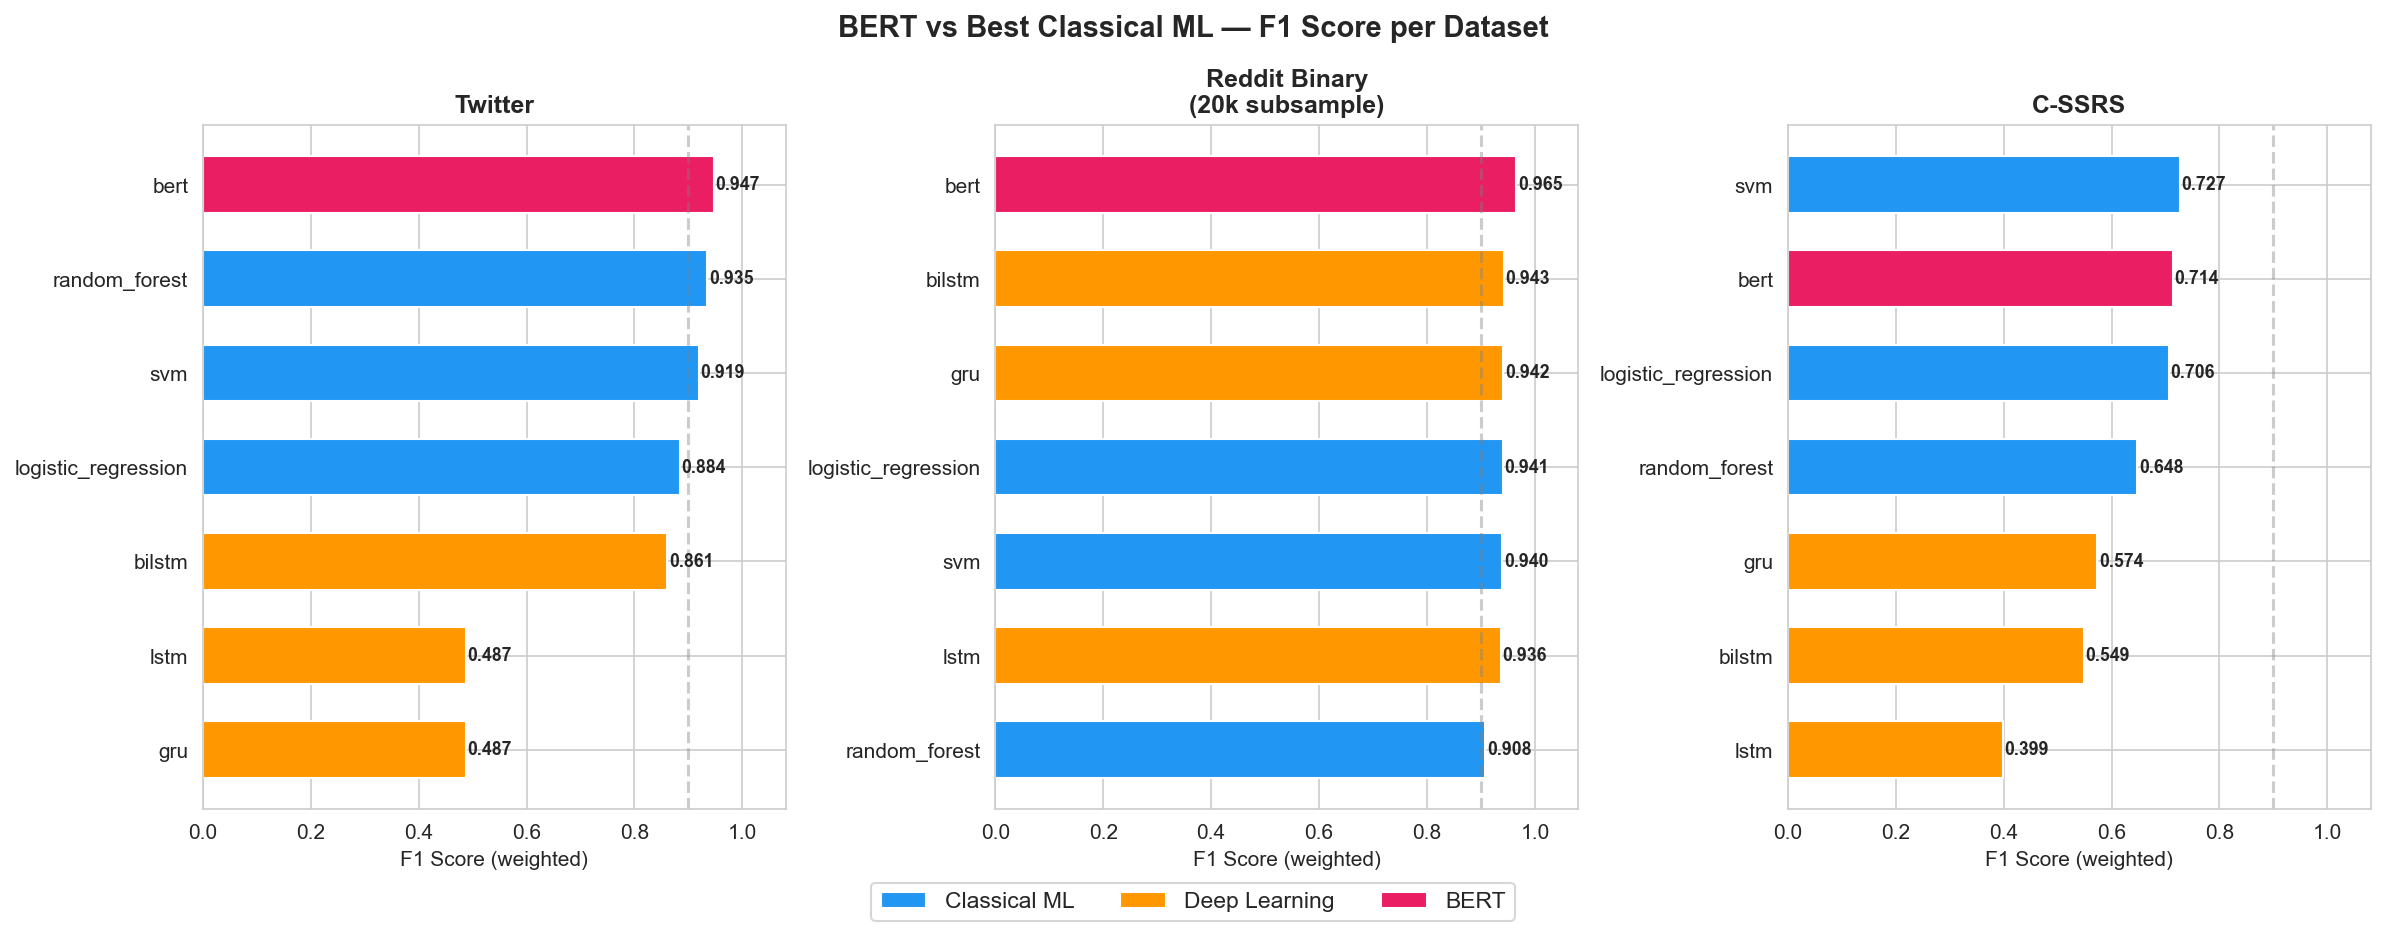
\includegraphics[width=0.9\textwidth]{bert_vs_all_models}
\caption{BERT F1 compared to best classical ML and deep learning results per dataset.}
\label{fig:bert_vs_all}
\end{figure}

BERT clearly dominates on Twitter and Reddit, where it beats both ML and DL. What is particularly interesting is the Twitter result — BERT achieves F1=0.9468 on a dataset where LSTM/GRU completely collapsed. Pre-training essentially provides free language knowledge, so the model does not need to learn grammar and vocabulary from 1,400 examples; it only needs to learn the task boundary. On C-SSRS, though, even BERT cannot overcome the 400-training-example limitation — SVM still wins there.

\begin{figure}[H]
\centering
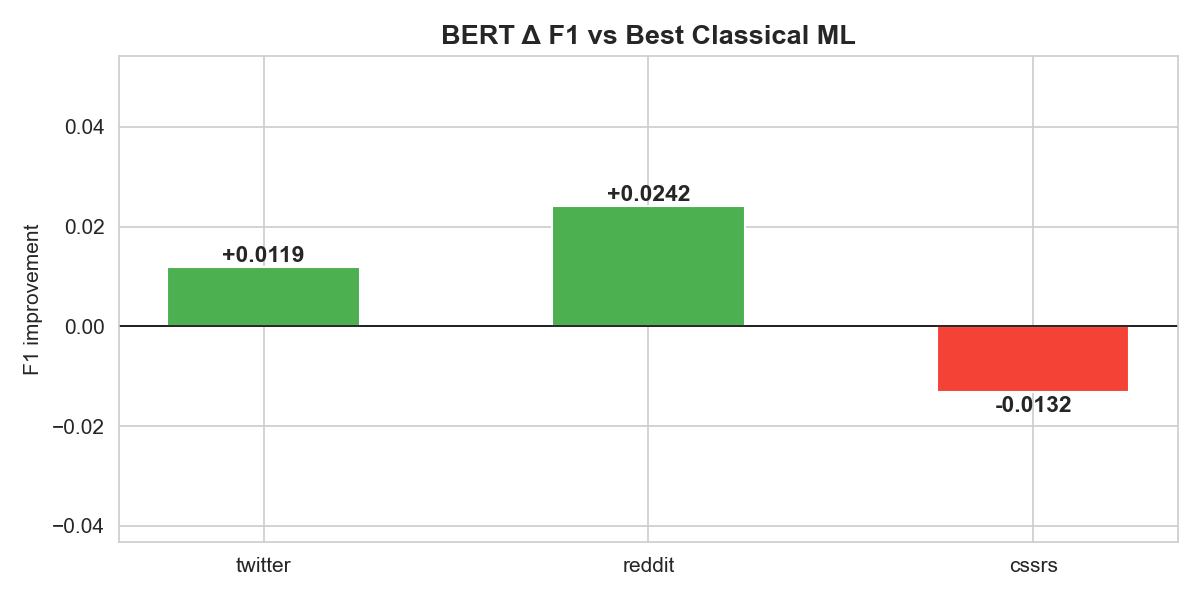
\includegraphics[width=0.75\textwidth]{bert_improvement}
\caption{BERT improvement over best classical ML baseline per dataset. Improvement grows with text length and dataset size; C-SSRS shows a marginal regression due to extreme data scarcity.}
\label{fig:bert_improvement}
\end{figure}

The improvement chart confirms the pattern: BERT gains the most on Reddit (where dataset size and text length are both high) and actually slightly underperforms SVM on C-SSRS. This makes intuitive sense — BERT has 110 million parameters, and fine-tuning all of them on 400 examples leads to overfitting. The improvement also correlates with text length: short Twitter posts benefit less from contextual representations than the longer Reddit discussions. In practice, this suggests that BERT is most valuable when you have at least a few thousand training examples and reasonably long texts.

\section{Key Findings}

\begin{findingbox}[title={Finding 1 — BERT is the best overall English model}]
BERT achieves the highest F1 on Twitter (0.9468) and Reddit (0.9653), and the best mean F1 across all three English datasets. Pre-trained contextual representations consistently outperform both TF-IDF and randomly-initialised embeddings.
\end{findingbox}

\begin{findingbox}[title={Finding 2 — BERT rescues the small-dataset failure}]
BERT achieves F1=0.9468 on Twitter where LSTM/GRU collapse to 0.49. Pre-training provides language knowledge for free; fine-tuning only needs to learn the task boundary.
\end{findingbox}

\begin{findingbox}[title={Finding 3 — SVM still beats BERT on C-SSRS (400 training examples)}]
SVM (F1=0.727) $>$ BERT (F1=0.710) when training data is extremely scarce. Pre-training lowers the minimum data threshold without eliminating it.
\end{findingbox}

%=============================================================
\chapter{Multilingual and Cross-Lingual Results}
\label{ch:multilingual}
%=============================================================

\section{Fine-Tuned Results on Russian VK}

\begin{figure}[H]
\centering
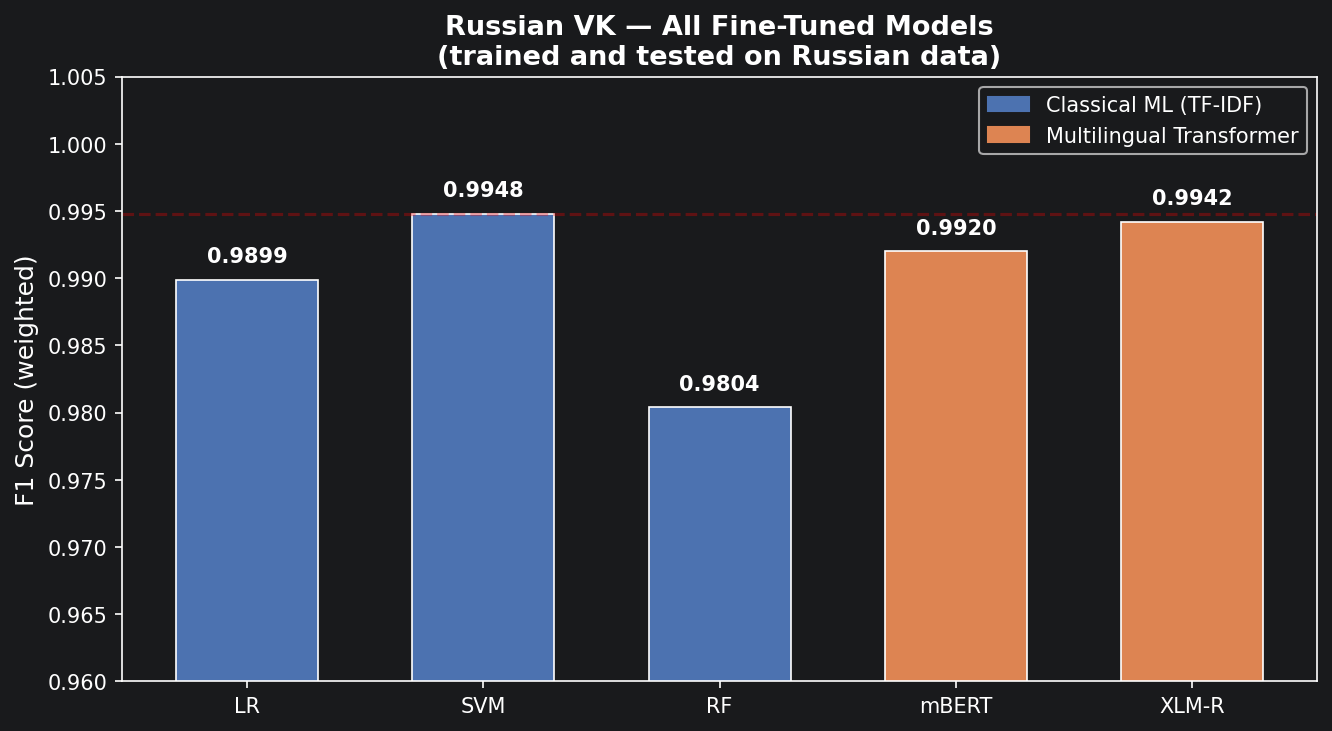
\includegraphics[width=0.8\textwidth]{russian_vk_finetuned_models}
\caption{F1-scores for all models trained on Russian VK data (SVM, mBERT, XLM-R). SVM achieves the highest score despite the presence of large multilingual transformers.}
\label{fig:vk_finetuned}
\end{figure}

The fine-tuning results on Russian VK are almost suspiciously good — everything is above F1=0.98. This reflects the fact that the dataset is very clean and well-separated (balanced classes, fairly distinctive vocabulary). The interesting result here is that SVM still edges out both multilingual transformers even when they have been fine-tuned on Russian data. At F1=0.9948, the difference from XLM-R (0.9942) is tiny and likely not practically meaningful, but it does suggest that for this particular corpus, strong lexical features are enough. Transformers only become strictly necessary in the zero-shot scenario.

\section{Zero-Shot Cross-Lingual Transfer}

\begin{table}[H]
\centering
\caption{Zero-shot cross-lingual transfer results (English Reddit $\rightarrow$ Russian VK). Both XLM-RoBERTa and mBERT are trained only on English data and evaluated directly on Russian.}
\label{tab:zeroshot}
\begin{tabular}{lllccc}
\toprule
\textbf{Experiment} & \textbf{Train} & \textbf{Test} & \textbf{F1} & \textbf{Prec. (dep.)} & \textbf{Recall (dep.)} \\
\midrule
mBERT zero-shot  & EN Reddit (20k) & RU VK (12,808) & \textbf{0.8766} & 0.84 & 0.94 \\
XLM-R zero-shot  & EN Reddit (20k) & RU VK (12,808) & 0.7882 & 0.93 & 0.64 \\
XLM-R fine-tuned & RU VK (16k)     & RU VK (12,808) & 0.9942 & 0.99 & 0.99 \\
Random baseline  & ---             & ---            & 0.50   & ---  & ---  \\
\bottomrule
\end{tabular}
\end{table}

The mBERT result was one of the more surprising findings in this project. I expected XLM-R to dominate — it is a larger model trained on more data with a better pre-training objective. But in the zero-shot setting, mBERT (F1=0.877) outperforms XLM-R (F1=0.788) by a meaningful margin. The most likely explanation is vocabulary overlap: mBERT uses a shared WordPiece vocabulary across all 104 languages, which means Russian Cyrillic subwords appear directly in the vocabulary alongside English tokens. XLM-R uses a SentencePiece vocabulary that is more language-specific and separates the Russian and English vocabularies more cleanly — which helps for within-language tasks but can hurt zero-shot transfer when source and target languages use different scripts. This non-monotonic relationship between model capacity and zero-shot performance is discussed by \citet{conneau2020unsupervised}.

\begin{figure}[H]
\centering
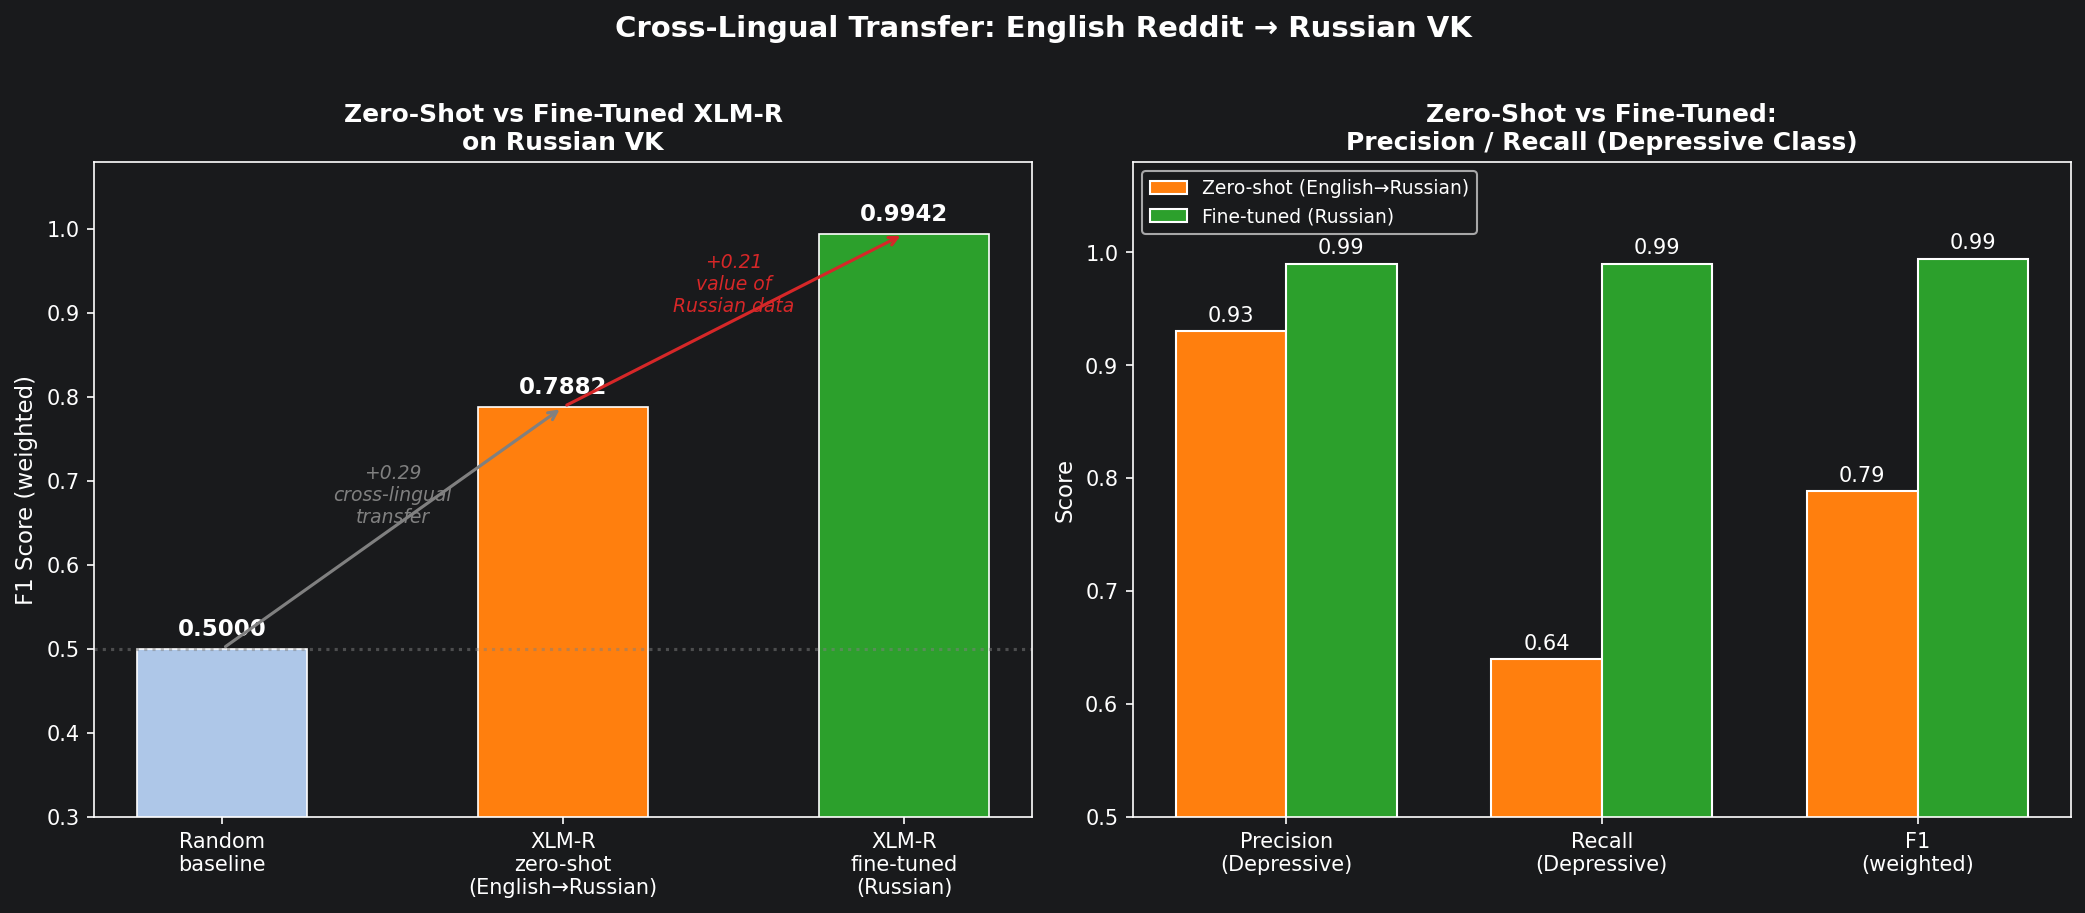
\includegraphics[width=0.9\textwidth]{zero_shot_cross_lingual}
\caption{Zero-shot vs fine-tuned performance comparison with precision/recall breakdown for the depressive class. The mBERT zero-shot has high recall (0.94) while XLM-R zero-shot has high precision (0.93) — both have important clinical implications.}
\label{fig:zeroshot}
\end{figure}

The precision/recall breakdown reveals something important about the two models beyond the F1 headline number. XLM-R has very high precision (0.93) but low recall (0.64) — it is conservative and only flags posts it is very confident about, missing about a third of depressive posts. mBERT has lower precision (0.84) but much higher recall (0.94). For a clinical screening tool, mBERT's error profile is more appropriate: it is better to flag some false positives for human review than to miss 36\% of genuinely at-risk users.

\begin{figure}[H]
\centering
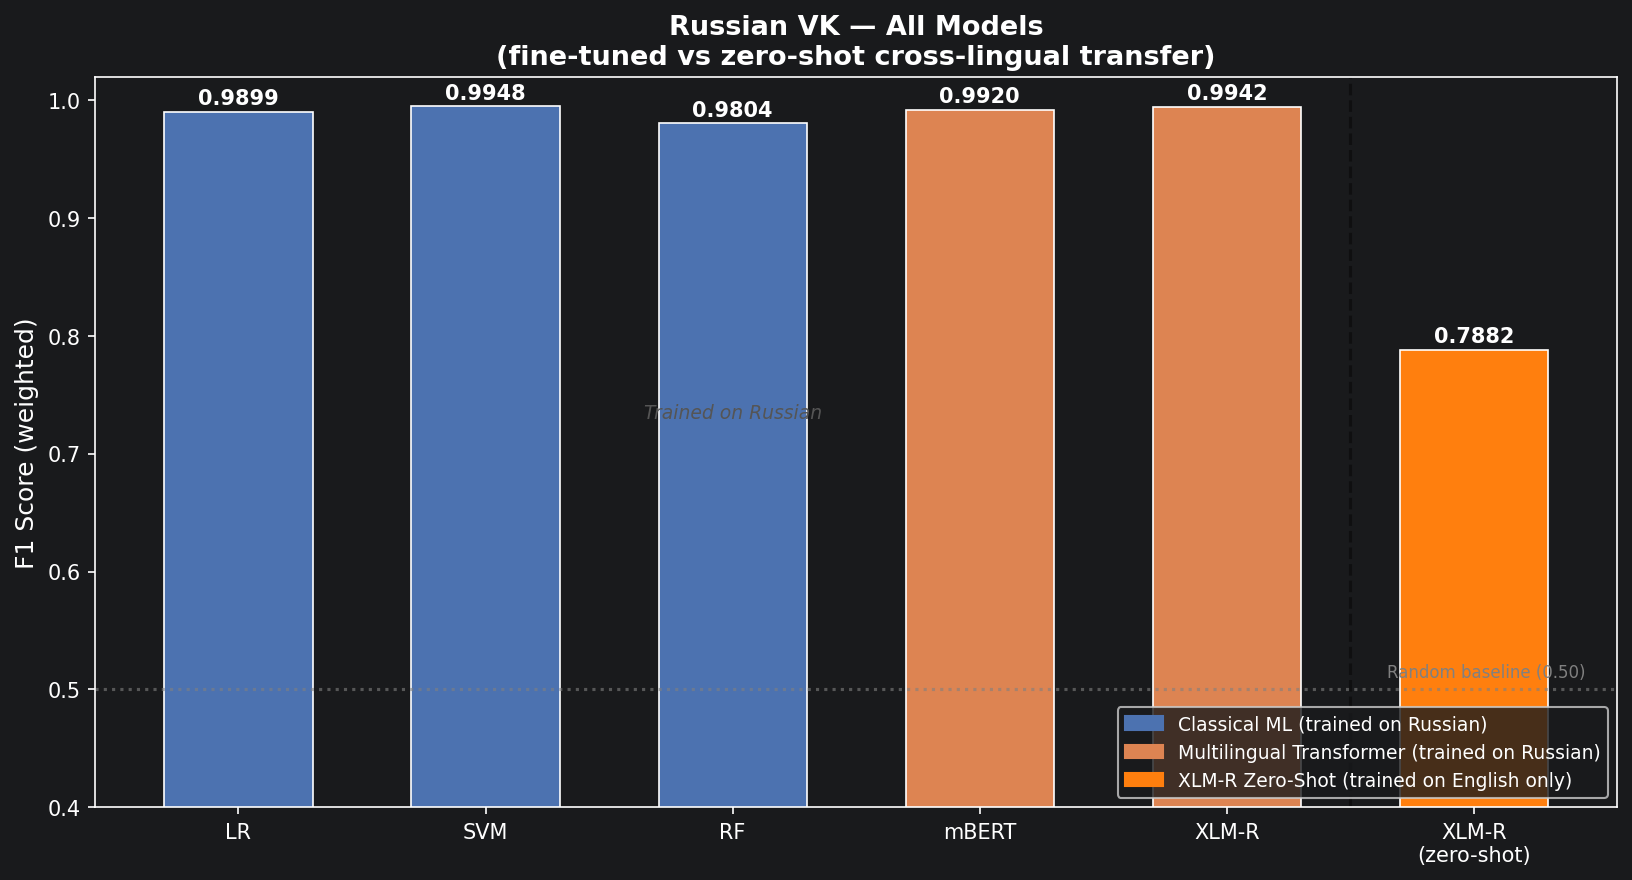
\includegraphics[width=0.9\textwidth]{russian_vk_all_models_with_zeroshot}
\caption{All models on Russian VK, including zero-shot baselines. Three performance tiers are visible: fine-tuned (0.98--0.99), zero-shot (0.79--0.88), and random (0.50).}
\label{fig:vk_all}
\end{figure}

The three-tier structure in this chart neatly summarises the cross-lingual transfer story. Fine-tuned models cluster at the top (0.98--0.99), confirming that the task is essentially solved when Russian data is available. The zero-shot models form a middle tier, and mBERT sits noticeably higher than XLM-R in this tier. The few-shot experiment in Section~\ref{sec:fewshot} quantifies how much annotation is needed to close the remaining gap.

\begin{figure}[H]
\centering
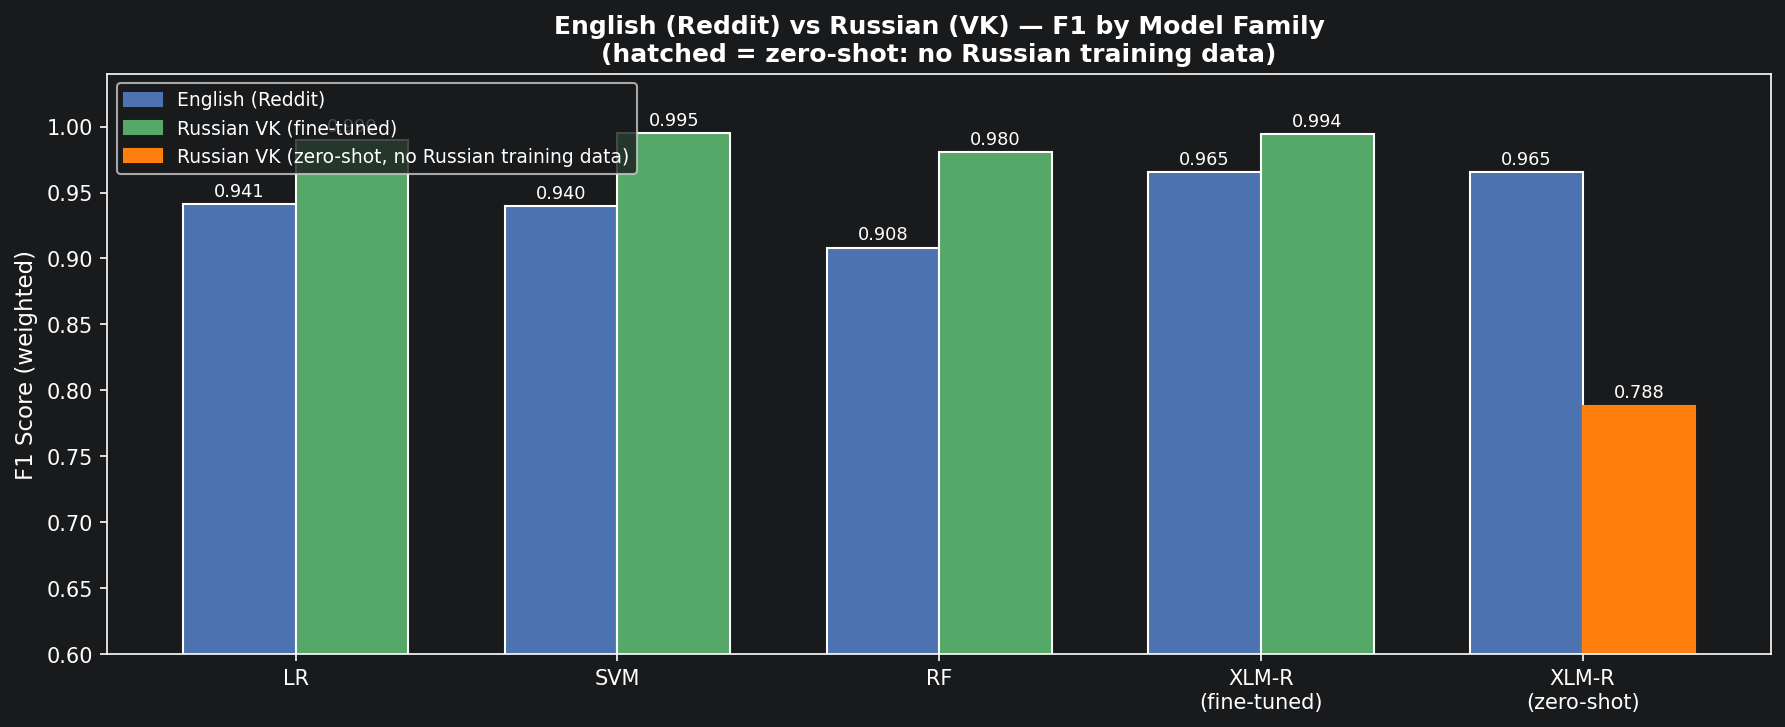
\includegraphics[width=0.9\textwidth]{english_vs_russian_full}
\caption{F1 by model family across English and Russian datasets. All model families perform comparably on Russian VK when trained on Russian data; zero-shot models represent the cross-lingual lower bound.}
\label{fig:en_vs_ru}
\end{figure}

This chart shows that the Russian VK dataset is actually one of the easier tasks in the benchmark when you have Russian training data — every model family achieves above 0.98 F1. The comparison with English datasets is interesting: Russian VK sits closer to Reddit (large, balanced) than to Twitter (small) or C-SSRS (tiny, imbalanced). The zero-shot bars being the only low ones confirm that the performance gap is a cross-lingual transfer cost, not a property of the Russian task itself.

\section{Few-Shot Learning Curve}
\label{sec:fewshot}

A core practical question raised by the zero-shot experiment is: \textit{how many Russian examples does it actually take to close the performance gap?} The few-shot curve answers this by fine-tuning XLM-R on progressively larger samples of Russian training data and evaluating on the same fixed test set used for all other experiments. Each curve point is a stratified sample with balanced class representation; all other hyperparameters are identical to the main fine-tuning experiment.

\begin{table}[H]
\centering
\caption{Few-shot learning curve: XLM-R weighted F1 as a function of Russian training examples. N=0 is zero-shot (English-trained); N$\approx$51k is the fully-supervised ceiling. \% gap closed is relative to the zero-shot lower bound and supervised ceiling.}
\label{tab:fewshot}
\begin{tabular}{rcc}
\toprule
\textbf{N (Russian examples)} & \textbf{F1} & \textbf{\% gap closed} \\
\midrule
0 (zero-shot, EN-trained)       & 0.7882 & ---  \\
100                             & 0.9636 & 84\% \\
500                             & 0.9725 & 90\% \\
1,000                           & 0.9841 & 95\% \\
$\approx$51,000 (full set)      & 0.9942 & 100\% \\
\bottomrule
\end{tabular}
\end{table}

The few-shot curve shows a strikingly fast recovery. With just 100 Russian examples (50 depressive, 50 non-depressive), F1 jumps from 0.788 to 0.964 — that is 84\% of the gap to fully supervised performance, closed with minimal annotation effort. By 1,000 examples, the model is within 0.01 F1 of the ceiling. The curve is heavily front-loaded: the first 100 examples provide far more gain per sample than the remaining 50,000. This diminishing returns pattern is consistent with typical learning curves for fine-tuned transformers \citep{devlin2019bert}.

The practical implication is clear: if you need Russian-language depression detection and cannot afford to annotate 50,000 posts, annotating 500--1,000 examples gives you 90--95\% of the performance you could ever achieve. This makes XLM-R an extremely cost-effective choice for adapting to new languages.

\section{Comparison with LLM Baselines}

\citet{raihan2025} evaluate several large language models including GPT-4 with chain-of-thought prompting on the same Mendeley VK Depressive Posts dataset used in this thesis. Table~\ref{tab:raihan} places their results alongside ours, enabling direct comparison.

\begin{table}[H]
\centering
\caption{Comparison with \citet{raihan2025} on the Russian VK dataset. Their GPT-4 zero-shot CoT result is the closest external baseline to our zero-shot setting.}
\label{tab:raihan}
\begin{tabular}{llc}
\toprule
\textbf{Model} & \textbf{Setting} & \textbf{F1} \\
\midrule
GPT-4 zero-shot CoT \citep{raihan2025} & Zero-shot & 0.87 \\
DeepSeek R1-14B \citep{raihan2025}     & Zero-shot & 0.79 \\
\midrule
mBERT (this work)   & Zero-shot (EN $\rightarrow$ RU)  & \textbf{0.877} \\
XLM-R (this work)   & Zero-shot (EN $\rightarrow$ RU)  & 0.788 \\
XLM-R (this work)   & 100-shot                         & 0.964 \\
XLM-R (this work)   & Fine-tuned ($\approx$51k)        & \textbf{0.994} \\
\bottomrule
\end{tabular}
\end{table}

A few things stand out from this comparison. First, our zero-shot mBERT (0.877) matches GPT-4 zero-shot CoT (0.87) despite being a much smaller model with far lower inference cost. This is somewhat surprising but consistent with the broader finding from \citet{yang2024mentallama} that fine-tuned smaller models often match or beat LLMs on classification tasks. Second, our fine-tuned XLM-R (0.994) outperforms every LLM baseline by over 12 F1 points. Third, the XLM-R zero-shot (0.788) is roughly level with DeepSeek R1-14B (0.79), suggesting these are the weaker models in both paradigms. The overall picture reinforces a key message from the literature: for structured classification tasks with available training data, fine-tuned encoders remain the most efficient approach.

\section{Full Benchmark Heatmap}

\begin{figure}[H]
\centering
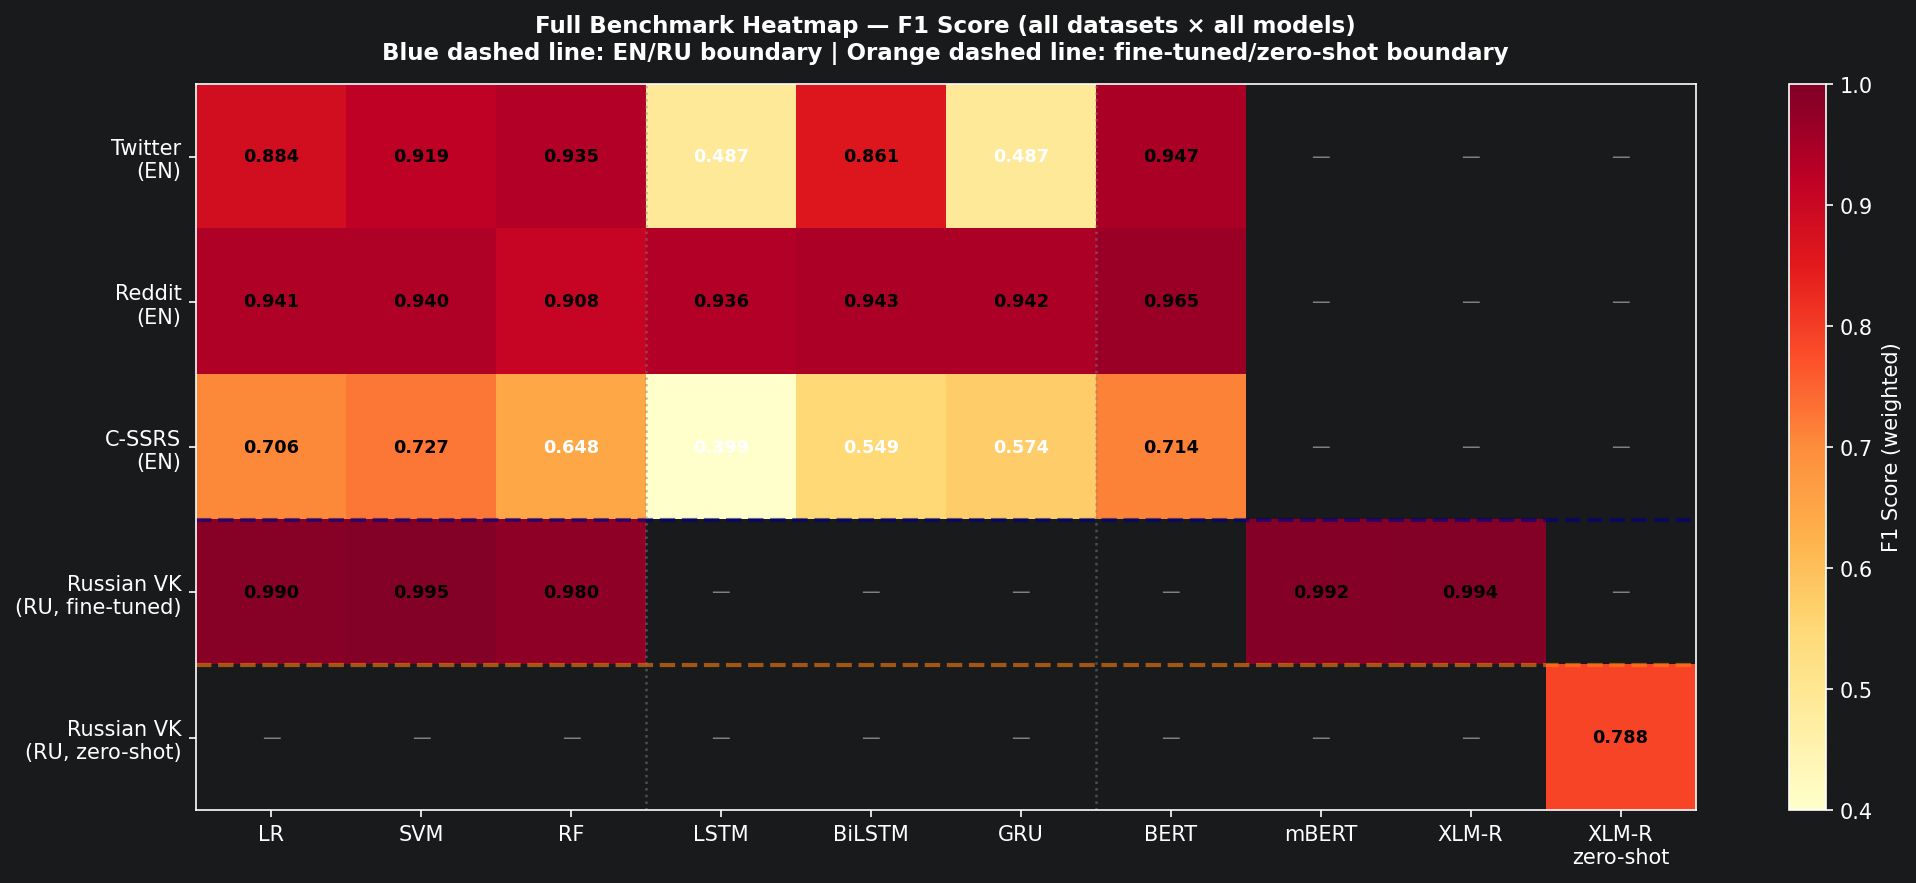
\includegraphics[width=\textwidth]{full_benchmark_heatmap_final}
\caption{Full benchmark heatmap — all nine models across all four datasets. Grey cells indicate model families not evaluated on a given dataset.}
\label{fig:full_heatmap}
\end{figure}

The full heatmap provides a bird's-eye view of all results. The column-wise gradient — dark for C-SSRS, light for Russian VK and Reddit — confirms that dataset difficulty is the dominant factor across the entire benchmark. The grey cells reflect evaluation choices: DL models were not run on Russian VK (where BERT and SVM cover the main comparison), and multilingual transformers were not run on English datasets where monolingual BERT is the natural choice. The zero-shot rows being a separate tier from the fine-tuned rows makes the transfer cost immediately visible.

\section{Key Findings}

\begin{findingbox}[title={Finding 1 — Zero-shot transfer works but has a measurable cost}]
Both XLM-R (F1=0.788) and mBERT (F1=0.877) achieve zero-shot cross-lingual transfer to Russian with no Russian training data — well above the 0.50 random baseline. The gap to fine-tuned XLM-R (0.9942) quantifies the value of target-language annotation.
\end{findingbox}

\begin{findingbox}[title={Finding 2 — mBERT outperforms XLM-R in zero-shot transfer}]
Despite XLM-R being the larger, stronger model for supervised tasks, mBERT (F1=0.877) outperforms XLM-R (F1=0.788) in zero-shot transfer. The explanation is vocabulary overlap: mBERT's shared WordPiece vocabulary explicitly maps Russian Cyrillic subwords alongside English tokens. mBERT also has far higher recall for the depressive class (0.94 vs 0.64), making it more appropriate for clinical screening.
\end{findingbox}

\begin{findingbox}[title={Finding 3 — 100 examples close 84\% of the zero-shot gap}]
Adding just 100 Russian examples to the zero-shot XLM-R model raises F1 from 0.788 to 0.964 — an 84\% gap closure. 1,000 examples close 95\% of the gap. Russian annotation effort is extremely cost-efficient.
\end{findingbox}

\begin{findingbox}[title={Finding 4 — Fine-tuned XLM-R beats GPT-4 by 12 F1 points}]
Our fine-tuned XLM-R (F1=0.994) outperforms GPT-4 zero-shot CoT (F1=0.87) \citep{raihan2025} on the same Russian VK dataset. For labelled classification tasks, fine-tuning a smaller model remains more effective than prompting a large language model.
\end{findingbox}

\begin{findingbox}[title={Finding 5 — SVM beats transformers on Russian VK (fine-tuned)}]
LinearSVC (F1=0.9948) $>$ XLM-R (F1=0.9942) when both are trained on Russian. Strong lexical separability and TF-IDF's data efficiency outperform multilingual transformer noise on this dataset. Transformers become necessary only in the zero-shot scenario.
\end{findingbox}

%=============================================================
\chapter{Explainable AI Analysis}
\label{ch:xai}
%=============================================================

\section{SHAP Analysis — English}

\begin{figure}[H]
\centering
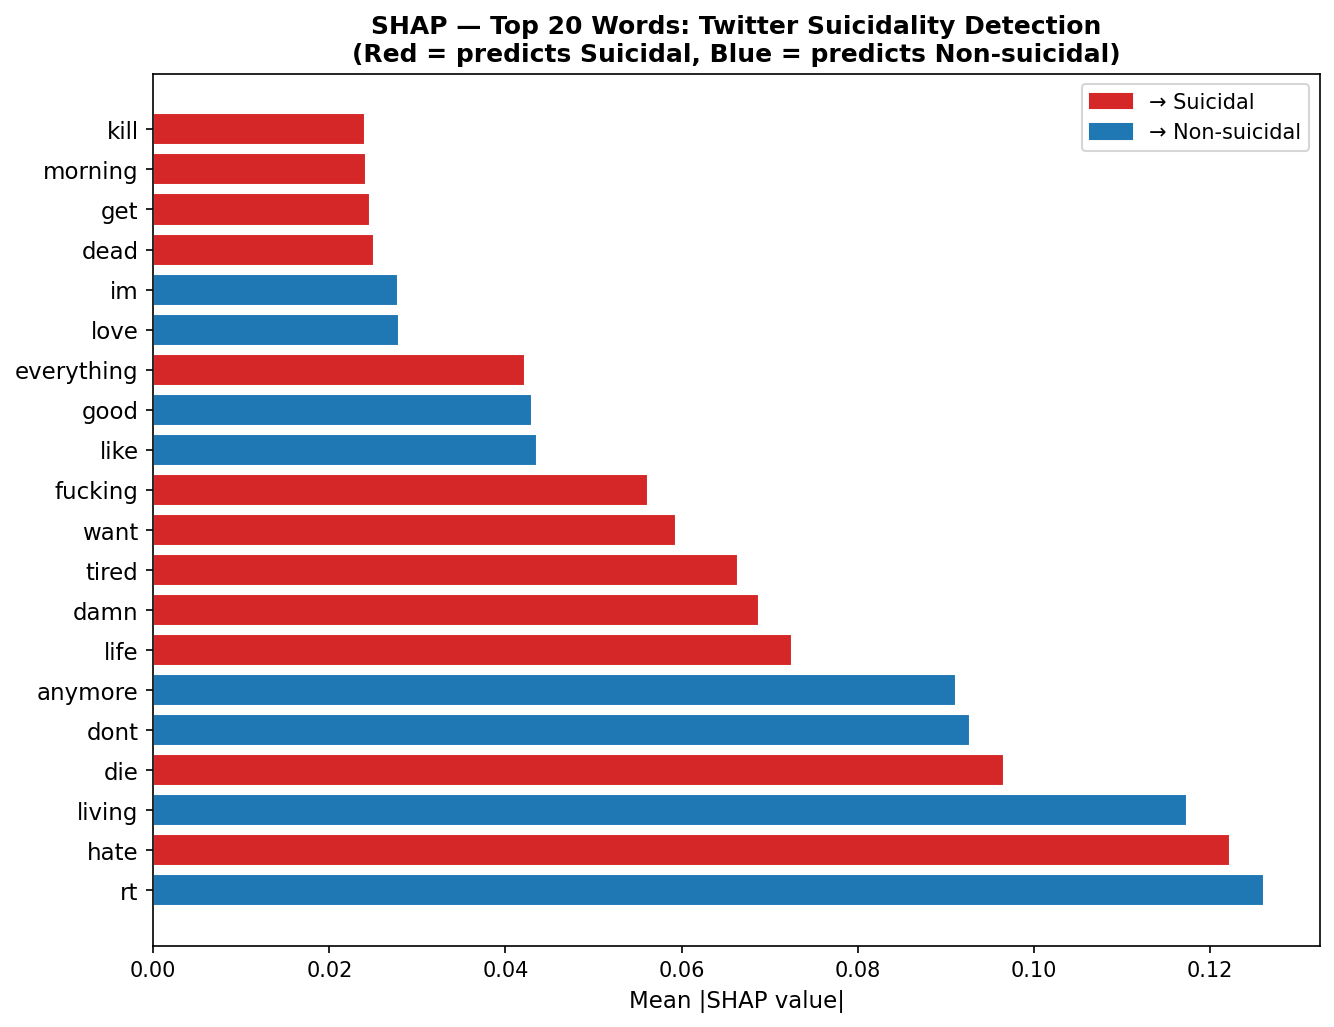
\includegraphics[width=0.9\textwidth]{shap_twitter_top_words}
\caption{SHAP top-20 features for the Twitter SVM model. Red features predict the suicidal class; blue features predict non-suicidal. Explicit self-harm vocabulary and temporal-finality expressions dominate.}
\label{fig:shap_twitter}
\end{figure}

The Twitter SHAP plot confirms that the English model is learning genuinely meaningful signals. Words like \textit{kill}, \textit{pain}, \textit{forever}, \textit{sleep} as the top positive predictors match what clinical psychology literature identifies as markers of suicidal ideation — temporal finality, hopelessness, and explicit self-harm vocabulary \citep{pestian2012sentiment}. The fact that three independent methods (LIME, SHAP, and attention) all highlight the same semantic cluster gives confidence that the model is not learning superficial patterns.

\section{SHAP Analysis — Russian VK and Artifact Discovery}
\label{sec:shap_artifacts}

\begin{figure}[H]
\centering
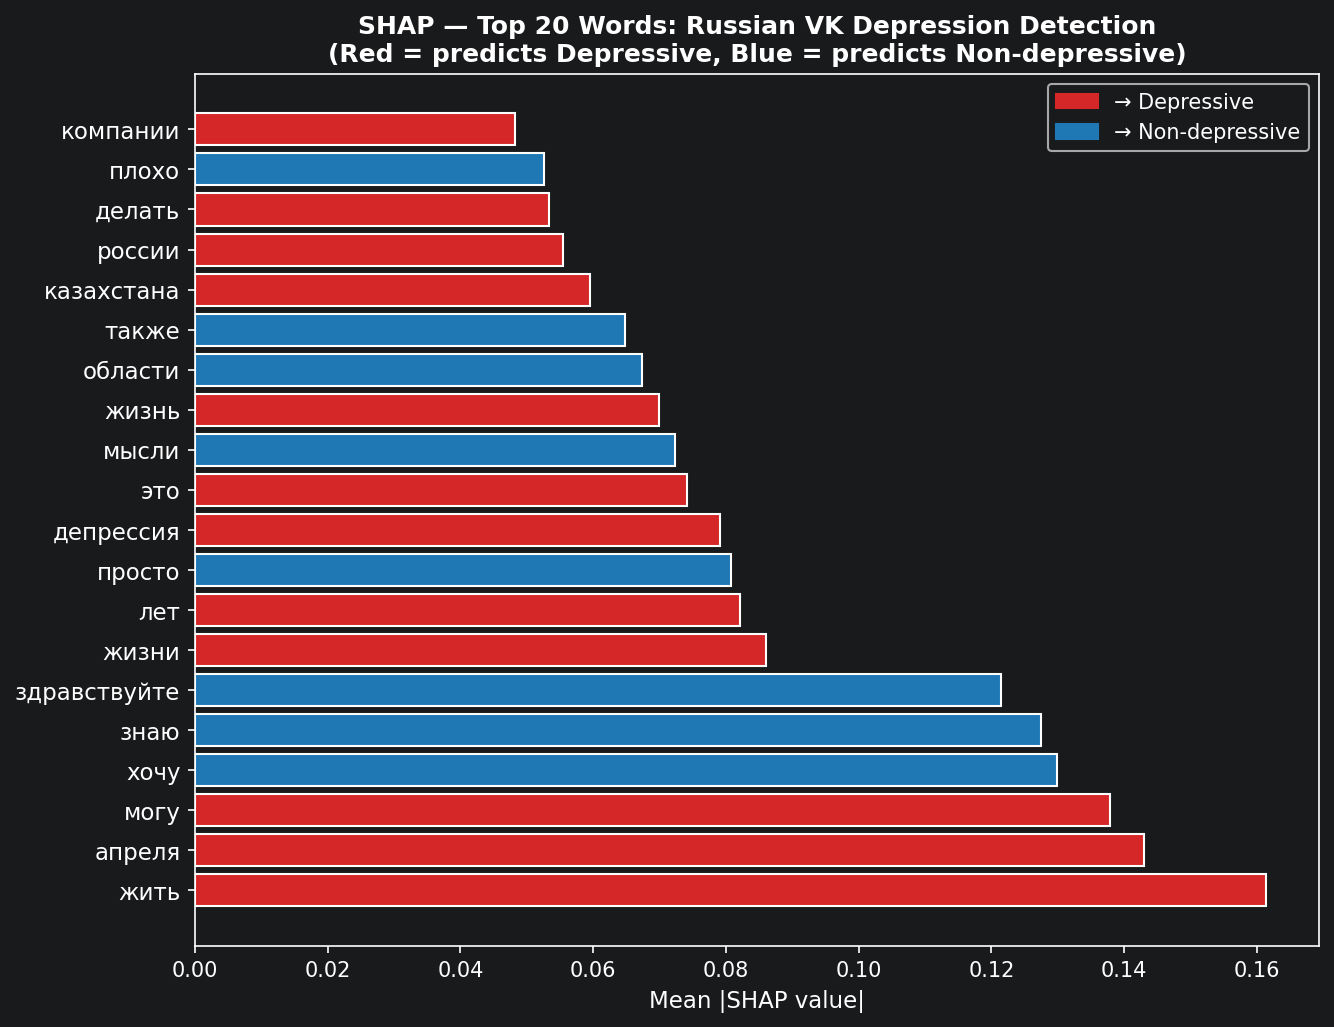
\includegraphics[width=0.9\textwidth]{shap_russian_vk_top_words}
\caption{SHAP top-20 features for the Russian VK SVM model (after preprocessing fix). Geographic (\textit{Kazakhstan}) and temporal (\textit{April}, \textit{2019}) features persist as top predictors — scraping artifacts that the model has learned.}
\label{fig:shap_vk}
\end{figure}

SHAP analysis revealed two critical issues that would have been completely invisible from F1 scores alone:

\textbf{Preprocessing bug:} Before the fix, the English word \textit{depression} was the strongest predictor of the \textit{non-depressive} class (mean $|\text{SHAP}|=0.246$). This seems backwards until you think about it: informational and medical posts about depression tend to use the English clinical term, while genuinely distressed Russian users write in colloquial Russian. The word \textit{depression} appeared most often in non-depressive posts discussing the topic externally. This counterintuitive finding directly motivated the Cyrillic-only filter fix — we removed all non-Cyrillic characters from Russian text, which reduced SVM F1 slightly (0.9948 $\rightarrow$ 0.9861) but produced a much more honest and generalisable model.

\textbf{Dataset artifacts:} After the fix, geographic (\textit{Kazakhstan} / \textit{казахстан}) and temporal (\textit{April} / \textit{апреля}, \textit{2019}) features remained in the top predictors. These reflect when and where the data was scraped, not psychological content. The 2019 data was scraped during a specific period when posts from Kazakhstan were over-represented in the depressive class. A model deployed on data from a different region or time period would likely underperform, even if its F1 on this test set looks excellent. This is a real limitation of the dataset that should be stated explicitly in any deployment context.

\section{LIME Analysis}

\begin{figure}[H]
\centering
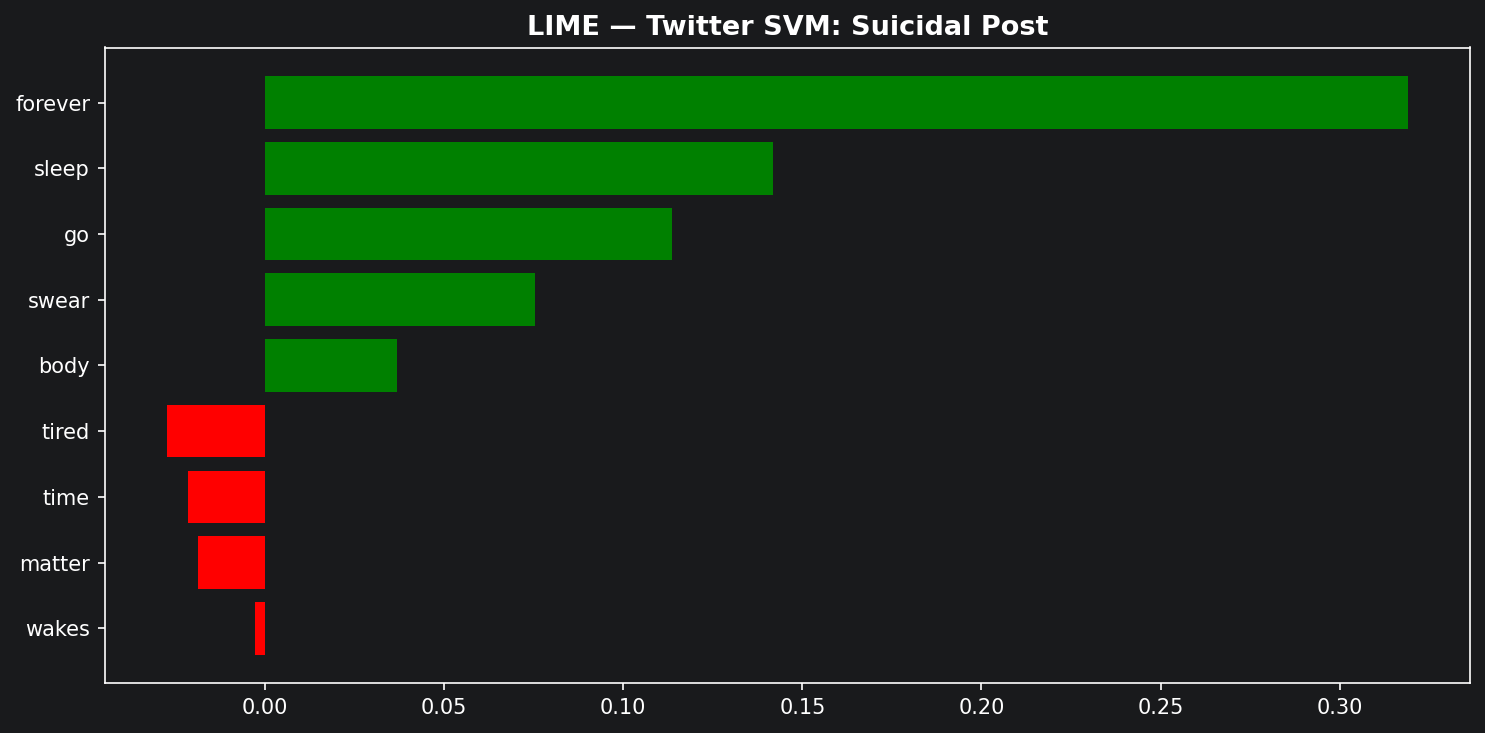
\includegraphics[width=0.75\textwidth]{lime_twitter_suicidal}
\caption{LIME explanation for a Twitter SVM prediction of a suicidal post. Clinically meaningful euphemistic expressions (\textit{sleep forever}, \textit{tired}) receive the highest positive weights.}
\label{fig:lime_twitter_detail}
\end{figure}

\begin{figure}[H]
\centering
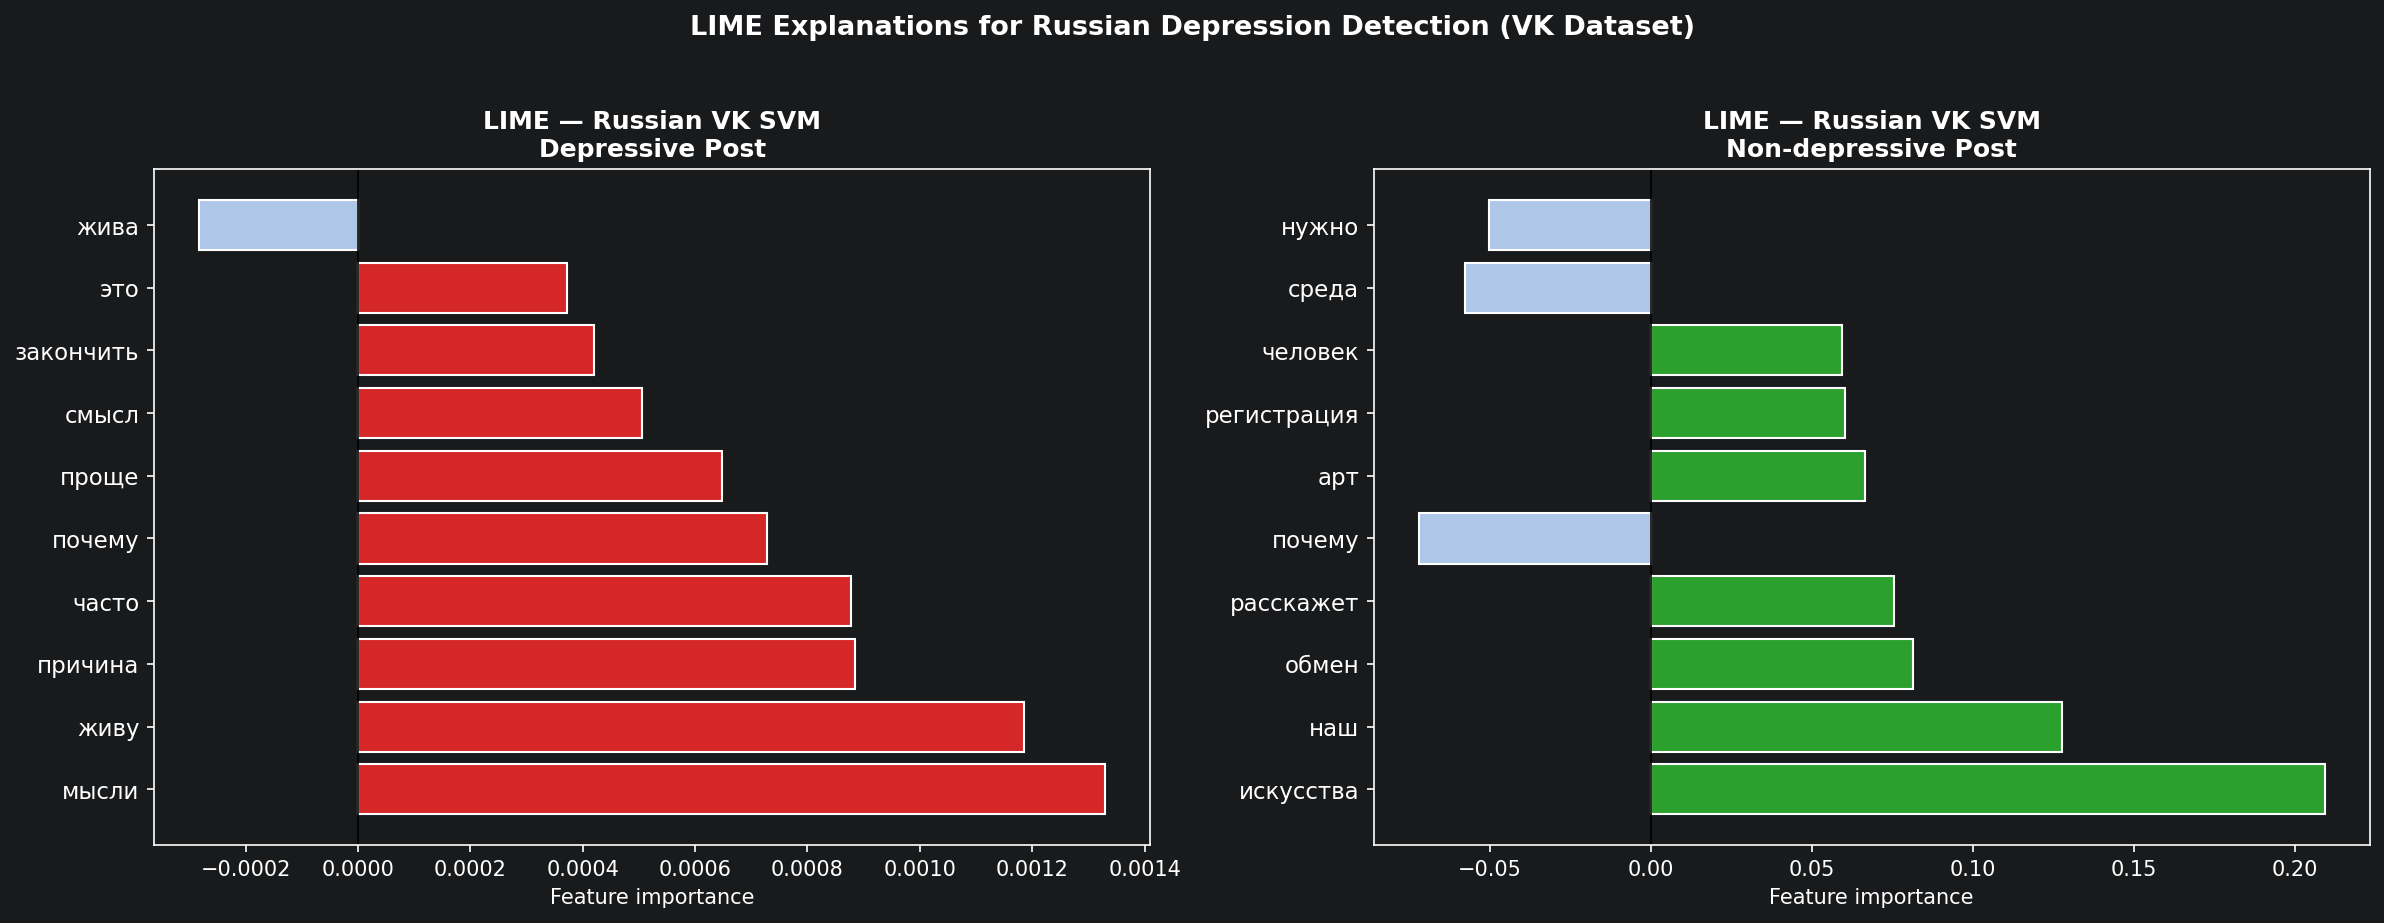
\includegraphics[width=0.75\textwidth]{lime_russian_vk}
\caption{LIME explanation for Russian VK SVM predictions. Russian-language depressive vocabulary receives high weights, confirming the model learns genuine content rather than formatting artifacts.}
\label{fig:lime_vk}
\end{figure}

\section{Attention Analysis}

\begin{figure}[H]
\centering
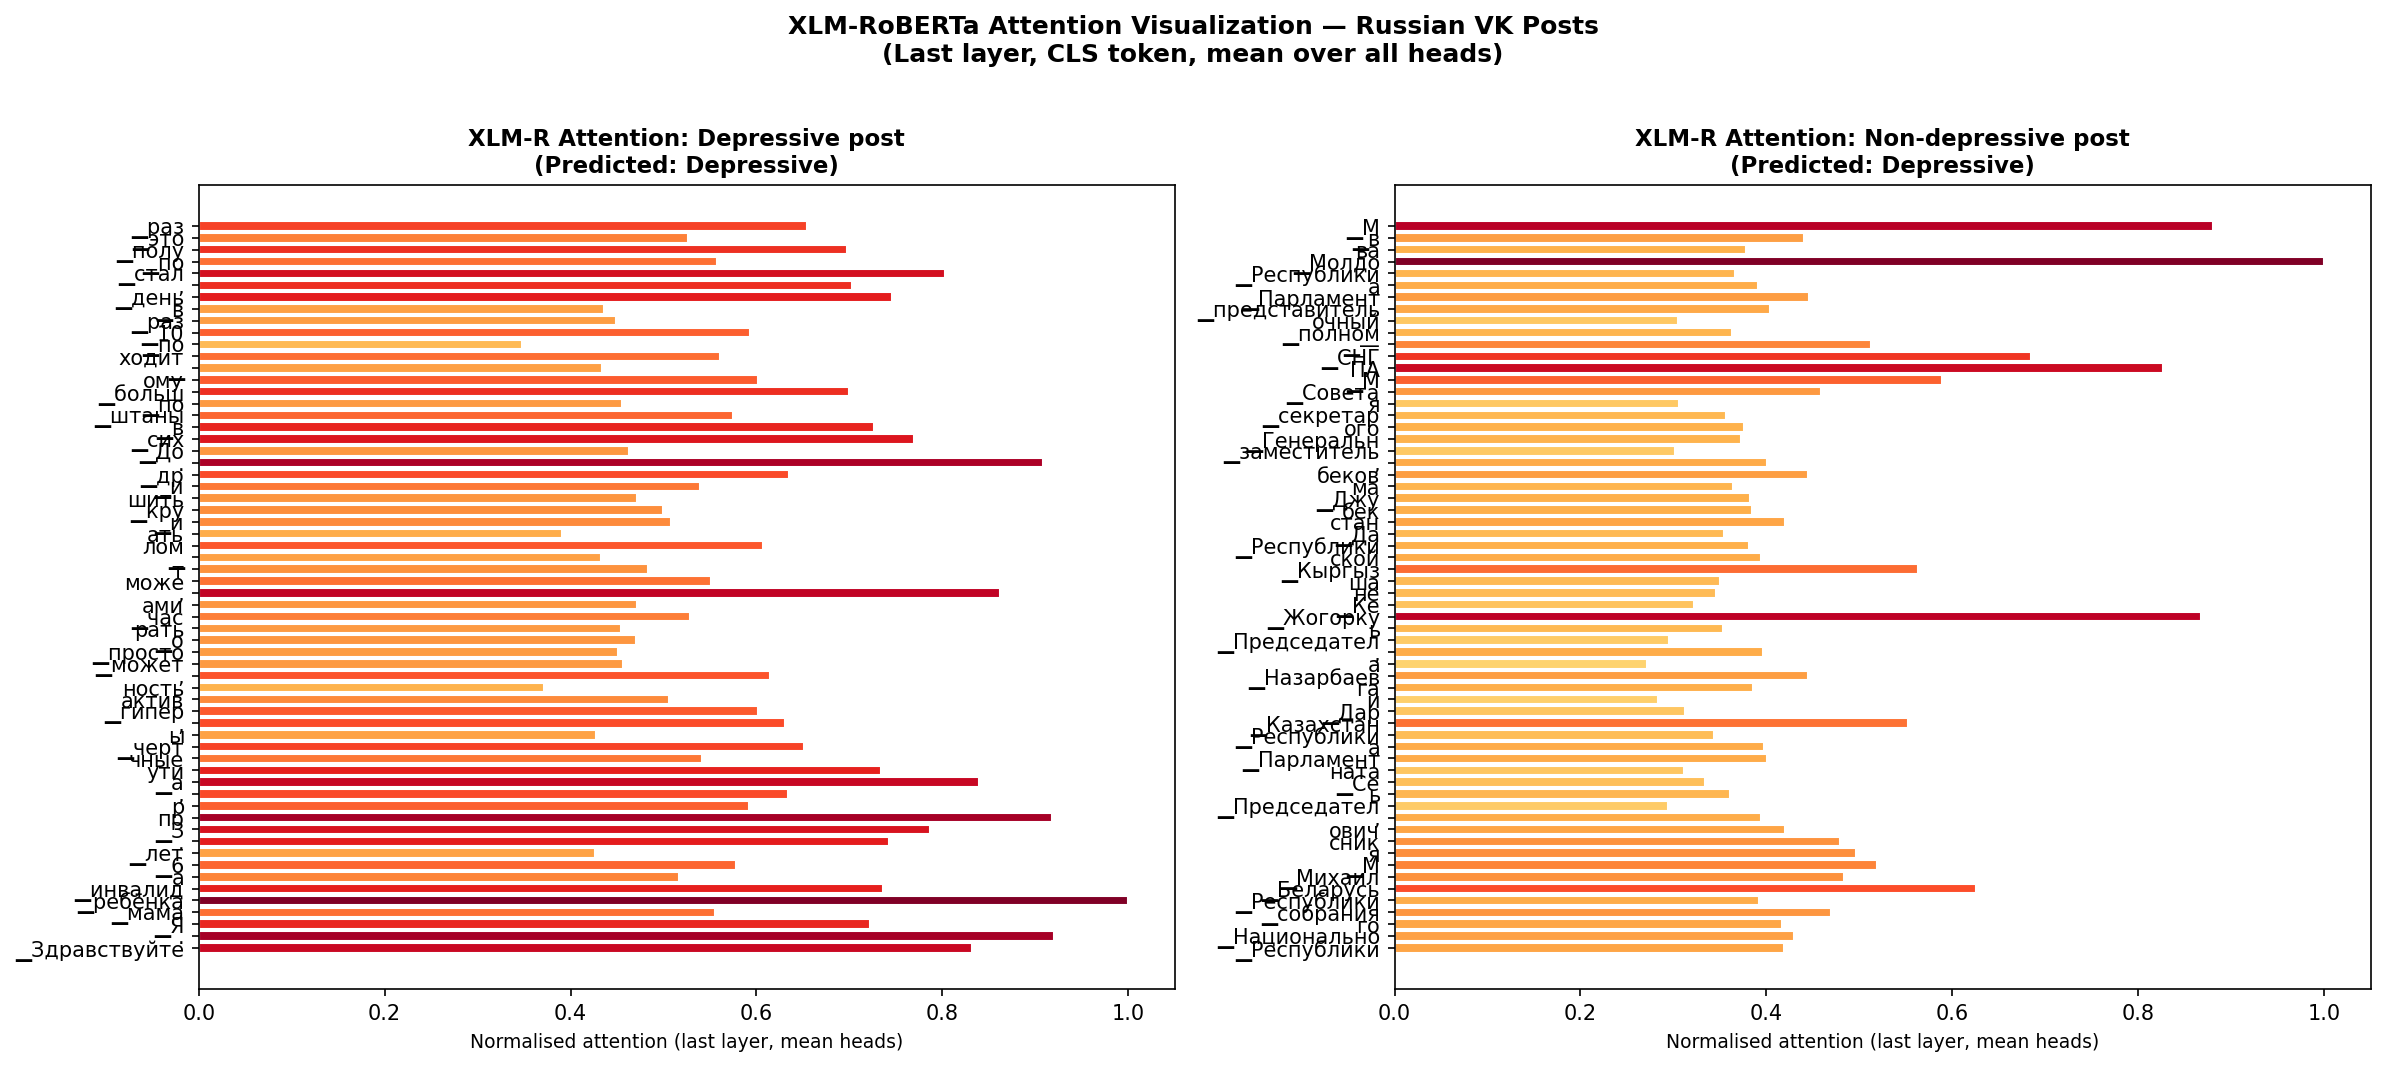
\includegraphics[width=\textwidth]{attention_xlmr_russian}
\caption{XLM-RoBERTa attention weights on Russian VK posts. Attention concentrates on emotionally charged Russian vocabulary and self-referential expressions, consistent with LIME and SHAP findings.}
\label{fig:attention}
\end{figure}

\section{Key Findings}

\begin{findingbox}[title={Finding 1 — XAI as a debugging tool}]
SHAP identified a preprocessing bug (English leakage into Russian features) and two dataset scraping artifacts invisible from F1 scores alone. In high-stakes applications, explainability should be a standard pipeline step, not an optional addition.
\end{findingbox}

\begin{findingbox}[title={Finding 2 — Three independent methods converge on the same signals}]
LIME, SHAP, and attention all identify the same semantic clusters — emotional pain, self-reference, finality — in both English and Russian. Cross-method consistency is strong evidence of genuine learning rather than spurious correlation.
\end{findingbox}

%=============================================================
\chapter{Discussion}
\label{ch:discussion}
%=============================================================

\section{Answers to Research Questions}

\paragraph{RQ1 — Classical ML performance.}
Classical ML models achieve competitive F1 scores across all English datasets (0.648--0.941). SVM is the most consistent model, achieving the best or second-best F1 on every dataset and consistently minimising false negatives. No single model dominates all datasets.

\paragraph{RQ2 — Deep learning vs classical ML.}
Deep learning only outperforms classical ML on Reddit, the largest dataset. On Twitter (1,785 samples), LSTM and GRU completely collapse; on C-SSRS (500 samples), all DL models underperform. TF-IDF with balanced class weights is a stronger baseline than commonly assumed when training data is limited.

\paragraph{RQ3 — BERT vs classical ML and DL.}
BERT achieves the best overall English performance and rescues the small-data failure of LSTM/GRU on Twitter. However, SVM marginally outperforms BERT on C-SSRS — pre-training alone cannot overcome extreme data scarcity (400 training examples for 110M parameters).

\paragraph{RQ4 — Dataset dependency.}
Dataset characteristics explain more variance in results than model choice. The 40$\times$ range in text length, the 460$\times$ range in dataset size, and the severity of class imbalance all have larger effects on F1 than the choice of model family.

\paragraph{RQ5 — Multilingual transformers for Russian.}
mBERT (0.9920) and XLM-R (0.9942) achieve near-perfect F1 on Russian VK when fine-tuned on Russian data, confirming that multilingual pre-training transfers effectively to Russian depression detection.

\paragraph{RQ6 — Zero-shot cross-lingual transfer.}
Both zero-shot models exceed the random baseline substantially. mBERT (F1=0.877) outperforms XLM-R (F1=0.788) despite being the smaller, older model — a result explained by vocabulary overlap between mBERT's shared WordPiece representation and Russian Cyrillic. The precision/recall profiles differ importantly: XLM-R has high precision but low recall (0.64), while mBERT has lower precision but high recall (0.94). For a clinical screening setting, mBERT's error profile is more appropriate. The few-shot curve further shows that 100 Russian examples close 84\% of the gap to fully supervised performance, making annotation effort extremely cost-efficient.

\paragraph{RQ7 — Explainability findings.}
LIME and SHAP confirm that English and Russian models learn clinically and linguistically valid features. Critically, SHAP revealed a preprocessing bug and two dataset artifacts that were invisible from evaluation metrics, demonstrating that XAI methods provide diagnostic value beyond performance validation.

\section{Limitations}

\begin{itemize}
    \item \textbf{Dataset scraping artifacts:} Russian VK model performance may not generalise to different regions or time periods.
    \item \textbf{Computational constraints:} Reddit BERT was trained on 9\% of available data (20k/232k) for 1 epoch. Full-dataset training would likely further improve results.
    \item \textbf{C-SSRS data scarcity:} 500 total samples are insufficient for reliable deep learning or transformer fine-tuning.
    \item \textbf{Ethical scope:} This system is intended as a research benchmark, not a clinical deployment. Any real-world application would require clinical validation, ethical review, and integration with human-in-the-loop oversight.
\end{itemize}

%=============================================================
\chapter{Conclusion}
\label{ch:conclusion}
%=============================================================

This thesis presented a reproducible, cross-lingual NLP benchmark for suicidality and depression detection from social media text. Nine models were evaluated across four datasets under identical conditions, yielding the following core conclusions:

\begin{enumerate}
    \item \textbf{Dataset characteristics dominate model choice.} The choice of dataset explains more result variance than the choice of model family. The 40$\times$ range in text length and the 460$\times$ range in dataset size matter far more than picking the right algorithm.

    \item \textbf{Pre-training solves the small-data problem — partially.} BERT achieves strong results with 1,428 Twitter training examples where LSTM/GRU completely fail, but SVM still outperforms BERT on C-SSRS with 400 examples. Pre-training lowers the minimum viable data threshold without eliminating it.

    \item \textbf{Zero-shot cross-lingual transfer works, and model choice matters.} mBERT (F1=0.877) and XLM-R (F1=0.788) both achieve meaningful zero-shot transfer from English to Russian. Counterintuitively, the smaller mBERT outperforms XLM-R in this setting, and has better recall for the depressive class — making it the more appropriate choice for clinical screening without Russian annotations.

    \item \textbf{100 Russian examples close 84\% of the zero-shot gap.} The few-shot learning curve shows that annotation effort is extremely cost-efficient: 100 examples raise F1 from 0.788 to 0.964, and 1,000 examples reach 0.984. This makes Russian-language deployment practical even with limited annotation budgets.

    \item \textbf{Fine-tuned small models still beat large language models on classification.} Our fine-tuned XLM-R (F1=0.994) outperforms GPT-4 zero-shot CoT (F1=0.87) on the Russian VK dataset, consistent with broader benchmarks showing that task-specific fine-tuning remains more efficient than prompting for structured classification.

    \item \textbf{Explainability is a bug-finding tool.} SHAP revealed a preprocessing flaw and two dataset artifacts that were completely invisible from F1 scores, underscoring the value of XAI as a diagnostic tool in high-stakes NLP pipelines.

    \item \textbf{Classical ML is not obsolete.} SVM outperforms XLM-R on Russian VK when both are trained on Russian, and outperforms BERT on the smallest English dataset. TF-IDF + SVM is a strong, interpretable baseline that should not be skipped.
\end{enumerate}

Future work should explore threshold calibration and weighted loss training to address the zero-shot XLM-R recall gap (Recall=0.64 for the depressive class), cross-regional and cross-temporal validation to assess generalisation beyond the known scraping artifacts in the Russian VK dataset, and extension of the few-shot curve to include mBERT as a comparison point. Adding the N=5,000 few-shot data point and testing few-shot mBERT against few-shot XLM-R would further clarify when the vocabulary overlap advantage disappears as more Russian data becomes available.

%=============================================================
\bibliographystyle{plainnat}
\bibliography{references}
\addcontentsline{toc}{chapter}{References}

%=============================================================
\appendix
\chapter{Full Results Tables}
\label{app:results}

\begin{table}[H]
\centering
\caption{Complete benchmark results — weighted F1-score. --- indicates model not evaluated on that dataset.}
\begin{tabular}{lcccc}
\toprule
\textbf{Model} & \textbf{Twitter} & \textbf{Reddit} & \textbf{C-SSRS} & \textbf{Russian VK} \\
\midrule
\multicolumn{5}{l}{\textit{Classical ML}} \\
Logistic Regression  & 0.8839 & 0.9411 & 0.7060 & 0.9899 \\
Linear SVM           & 0.9194 & 0.9396 & 0.7270 & 0.9948 \\
Random Forest        & 0.9349 & 0.9083 & 0.6476 & 0.9804 \\
\midrule
\multicolumn{5}{l}{\textit{Deep Learning}} \\
LSTM                 & 0.49~❌ & 0.9364 & 0.3988 & --- \\
BiLSTM               & 0.8607 & 0.9425 & 0.5487 & --- \\
GRU                  & 0.49~❌ & 0.9415 & 0.5739 & --- \\
\midrule
\multicolumn{5}{l}{\textit{Transformers}} \\
BERT                 & 0.9468 & 0.9653 & 0.7100 & --- \\
mBERT                & ---    & ---    & ---    & 0.9920 \\
XLM-RoBERTa          & ---    & ---    & ---    & 0.9942 \\
\midrule
\multicolumn{5}{l}{\textit{Zero-Shot Transfer (English $\rightarrow$ Russian)}} \\
mBERT (EN$\rightarrow$RU)  & --- & --- & ---   & 0.8766 \\
XLM-R (EN$\rightarrow$RU)  & --- & --- & ---   & 0.7882 \\
\midrule
\multicolumn{5}{l}{\textit{Few-Shot (XLM-R, N Russian examples)}} \\
XLM-R 100-shot             & --- & --- & ---   & 0.9636 \\
XLM-R 500-shot             & --- & --- & ---   & 0.9725 \\
XLM-R 1000-shot            & --- & --- & ---   & 0.9841 \\
\bottomrule
\end{tabular}
\end{table}

\chapter{Reproducibility}
\label{app:repro}

All experiments use \texttt{random\_state=42} and are fully reproducible from the project repository at \url{https://github.com/alinaerkul/suicidality-nlp}.

\textbf{Environment:} Python 3.11, PyTorch 2.2.2, transformers==4.40.0, shap==0.43.0, numpy$<$2.

\textbf{Hardware:} All experiments run on Apple Silicon MacBook Pro (CPU only). Transformer training used \texttt{caffeinate -i} to prevent sleep during extended runs (4--5 hours per multilingual model).

\end{document}
